\documentclass[twoside,11pt]{article}
\usepackage{jair, theapa, rawfonts}

\usepackage{amsmath}
\usepackage{amssymb}
\usepackage{amsfonts}
\usepackage{amsthm}
\usepackage{galois}
\usepackage{stmaryrd}
\usepackage{algorithm}
\usepackage{algpseudocode}
\usepackage[all,pdf]{xy}
\usepackage{lmodern,amssymb}
\usepackage[makeroom]{cancel}

\usepackage{tikz}
\usetikzlibrary{shapes}
\usetikzlibrary{backgrounds}

\newtheorem{theorem}{Theorem}
\newtheorem{lemma}{Lemma}
\newtheorem{definition}{Definition}
\newtheorem{proposition}{Proposition}

\newcommand{\B}{\mathbb{B}}
\newcommand{\D}{\mathcal{D}}
\newcommand{\Q}{\mathbb{Q}}
\newcommand{\R}{\mathbb{R}}
\newcommand{\I}{\mathcal{I}}
\newcommand{\N}{\mathbb{N}}
\newcommand{\FP}{\mathcal{FP}}
\newcommand{\PFP}{\powerset{\FP}}
\newcommand{\PD}{\powerset{\D}}

\newcommand{\abs}[1]{\widehat{#1}}
\newcommand{\absvec}[1]{\widehat{\uppercase{#1}}}
\newcommand{\A}{\mathcal{A}}

\newcommand{\powerset}[1]{\raisebox{.15\baselineskip}{\Large\ensuremath{\wp}}(#1)}
\newcommand{\powersett}[1]{\raisebox{.15\baselineskip}{\Large\ensuremath{\wp}}_{\ge 1}(#1)}
\DeclareMathOperator*{\argmax}{arg\,max}
\DeclareMathOperator*{\argmin}{arg\,min}
\DeclareMathOperator*{\sigmoid}{sigmoid}
\DeclareMathOperator*{\softmax}{softmax}

\newcommand*{\Not}{\textbf{not }}
\newcommand*\Let[2]{\State #1 $\gets$ #2}
\newcommand*\Yield[1]{\State \textbf{yield} #1}
\algblockdefx[ForEach]{ForEach}{EndForEach}[1]{\textbf{for each} #1 \textbf{do}}{\textbf{end for}}

\newif\ifboldnumber
\newcommand{\boldnext}{\global\boldnumbertrue}

% Default definition is \footnotesize#1:
\algrenewcommand\alglinenumber[1]{%
  \footnotesize\ifboldnumber\bfseries\fi\global\boldnumberfalse#1:}
  
\jairheading{vv}{yyyy}{ppp-ppp}{11/2022}{mm/yyyy}
\ShortHeadings{Finding Minimum-Cost Explanations for Predictions made by Tree Ensembles}
{Törnblom, Karlsson, \& Nadjm-Tehrani}
\firstpageno{1}


\begin{document}

\title{Finding Minimum-Cost Explanations for Predictions made by Tree Ensembles}

\author{%
  \name John Törnblom \email john.tornblom@saabgroup.com \\
  \name Emil Karlsson \email emil.karlsson1@saabgroup.com \\
  \addr Saab AB,\\
        Bröderna Ugglas gata, Linköping, Sweden \\
  \name Simin Nadjm-Tehrani \email simin.nadjm-tehrani@liu.se \\
  \addr Dept. of Computer and Information Science,\\
        Linköping University, Linköping, Sweden
}
           
% For research notes, remove the comment character in the line below.
% \researchnote

\maketitle

%%%%%%%%%%%%%%%%%%%%%%%%%%%%%%%%%%%%%%%%%%%%%%%%%%%%%%%%%%%%%%%%%%%%%%%%%%%%%%%%
\begin{abstract}
The ability to explain why a machine learning model arrives at a particular 
prediction is crucial when used as decision support by human operators of 
critical systems. The provided explanations must be provably correct, and 
preferably without redundant information, called minimal explanations. 
In this paper, we aim at finding explanations for predictions made by tree 
ensembles that are not only minimal, but also minimum with respect to a cost 
function. 
%%%%%%%%%%%%%%%%%%%%%%%%%%%%%%%%%%%%%%%%%%%%%%%%%%%%%%%%%%%%%%%%%%%%%%%%%%%%%%%%
To this end, we first present a highly efficient oracle that can determine the 
correctness of explanations, surpassing the runtime performance of current 
state-of-the-art alternatives by several orders of magnitude when computing
minimal explanations. 
%%%%%%%%%%%%%%%%%%%%%%%%%%%%%%%%%%%%%%%%%%%%%%%%%%%%%%%%%%%%%%%%%%%%%%%%%%%%%%%%
Secondly, we adapt an algorithm called MARCO from related works (calling it
m-MARCO) for the purpose of computing a single minimum explanation per
prediction, and demonstrate an overall speedup factor of two compared to the
MARCO algorithm which enumerates all minimal explanations.
%%%%%%%%%%%%%%%%%%%%%%%%%%%%%%%%%%%%%%%%%%%%%%%%%%%%%%%%%%%%%%%%%%%%%%%%%%%%%%%%
Finally, we study the obtained explanations from a range of use cases, leading
to further insights of their characteristics. In particular, we observe that
in several cases, there are more than 100,000 minimal explanations to choose
from for a single prediction. In these cases, we see that only a small portion
of the minimal explanations are also minimum, and that the minimum explanations
are significantly less verbose, hence motivating the aim of this work. 
\end{abstract}

%%%%%%%%%%%%%%%%%%%%%%%%%%%%%%%%%%%%%%%%%%%%%%%%%%%%%%%%%%%%%%%%%%%%%%%%%%%%%%%%
\section{Introduction}
\label{sec:introduction}
In many practical applications of machine learning, the ability to explain why
a prediction model arrives at a certain decision is crucial~\shortcite{Hadji21}.
Although significant progress has been made to understand the intricacies of 
machine learning systems and how their predictions can be 
explained~\shortcite<for a comprehensive survey, see e.g.,>{Ras22,Kaur22}, 
there are still open research questions. In this work, we are concerned with the 
use of machine learning models in critical decision support systems such as 
medical diagnosis and flight management systems, where a human acts in a loop,
working together with the system to make critical decisions. In such cases,
explanations for predictions may enable their system operators to make informed 
interventions of autonomous actions when explanations appear unjustified. More
specifically, we aim at providing explanations that are provably correct and 
without redundant information for predictions made by a class of machine 
learning models called tree ensembles.
%%%%%%%%%%%%%%%%%%%%%%%%%%%%%%%%%%%%%%%%%%%%%%%%%%%%%%%%%%%%%%%%%%%%%%%%%%%%%%%%

To illustrate the notion and usefulness of such explanations, consider a 
fictive bank-loan application support system, realized by the simple decision
tree depicted by Figure~\ref{fig:bankloan}.

\begin{figure}[ht]
  \centering
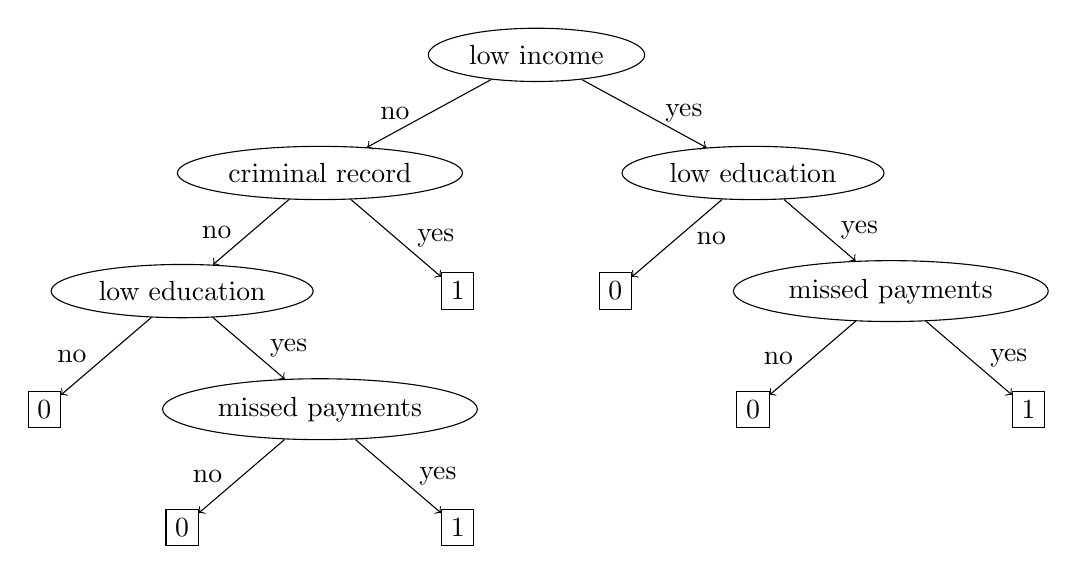
\begin{tikzpicture}[nodes={ellipse,draw}, ->, scale=1]
    \tikzstyle{every node}=[draw=black, ellipse, align=center, thin]
    \tikzstyle{level 1}=[level distance=15mm, sibling distance=55mm]
    \tikzstyle{level 2}=[sibling distance=35mm] 
    \node {low income}
        child {node {criminal record}
            child {node {low education}
                child {node[rectangle] {0}
                    edge from parent node[left,draw=none] {no}
                }
                child {node {missed payments}
                    child {node[rectangle] {0}
                        edge from parent node[left,draw=none] {no}
                    }
                    child {node[rectangle] {1}
                        edge from parent node[right,draw=none] {yes}
                    }
                    edge from parent node[right,draw=none] {yes}
                }
                edge from parent node[left,draw=none] {no}
            }
            child {node[rectangle] {1}
                edge from parent node[right,draw=none] {yes}
            }
            edge from parent node[left,draw=none] {no}
        }
        child {node {low education}
            edge from parent 
            child {node[rectangle] {0}
                edge from parent node[right,draw=none] {no}
            }
            child {node {missed payments}
                child {node[rectangle] {0}
                    edge from parent node[left,draw=none] {no}
                }
                child {node[rectangle] {1}
                    edge from parent node[right,draw=none] {yes}
                }
                edge from parent node[right,draw=none] {yes}
            }
            edge from parent node[right,draw=none] {yes}
        }
        ;
  \end{tikzpicture}
  \caption{A fictive bank-loan application processing system, where a 
           positive outcome indicates that the applicant should be denied a
           loan.}
  \label{fig:bankloan}
\end{figure}
%%%%%%%%%%%%%%%%%%%%%%%%%%%%%%%%%%%%%%%%%%%%%%%%%%%%%%%%%%%%%%%%%%%%%%%%%%%%%%%%
Suppose the system processes a particular applicant with a low income, low 
education, no criminal records, and a couple of missed payments, and the 
system denies the applicant a bank-loan. When explaining to the applicant 
why the requested loan is denied, information about criminal records may be
omitted since that particular feature does not contribute to the outcome of 
the prediction. Furthermore, if the applicant requests a new assessment after 
getting a salary raise (so that the applicant no longer has a low income), the 
system would respond the same. Consequently, an explanation only needs to 
include information about two of the four features; low education and missed
payments. We say that explanations that are correct and without redundant
information are minimal. Typically, there are several minimal explanations to
choose from, potentially hundreds of thousands for large systems. By 
associating each minimal explanation with a cost computed by a domain-specific
cost function, we can order them to find one that is most desirable for the 
problem at hand, called a minimum explanation. To this end, this paper 
contributes with the following.

%%%%%%%%%%%%%%%%%%%%%%%%%%%%%%%%%%%%%%%%%%%%%%%%%%%%%%%%%%%%%%%%%%%%%%%%%%%%%%%%
\begin{itemize}
    \item We formalize a sound and complete oracle for determining the 
          correctness of an explanation in the abstract interpretation 
          framework, designed specifically for tree ensembles.
          
    \item We demonstrate the performance of our oracle in a case study from
          related work that computes minimal explanations, and conclude an 
          overall speedup factor of 2,400 compared to current state-of-the-art.
          
    \item We demonstrate that, in the presence of a highly efficient oracle, 
          it is possible to enumerate all minimal explanations for several 
          predictions made by non-trivial tree ensembles.

    \item We propose an algorithm m-MARCO which is an adaptation of the MARCO 
          algorithm from related work~\shortcite{Liffiton16} for the purpose 
          of computing an explanation that is minimum, and demonstrate 
          an overall speedup factor of two compared to the MARCO algorithm
          which enumerates all minimal explanations. 
          
    \item We demonstrate that m-MARCO is significantly faster than a branch 
          and bound approach used in some SMT solvers to compute 
          counter-examples of unsatisfiable formulas.
\end{itemize}
We also provide\footnote{Published online, should the paper be accepted.} 
an implementation of our algorithms, together with logs and automated scripts 
to reproduce our results.

%%%%%%%%%%%%%%%%%%%%%%%%%%%%%%%%%%%%%%%%%%%%%%%%%%%%%%%%%%%%%%%%%%%%%%%%%%%%%%%%
The rest of this paper is structured as follows. Section~\ref{sec:prel}
provides preliminaries on the computation of minimal and minimum explanations,
the MARCO algorithm, decision trees and tree ensembles, and abstract 
interpretation. In Section~\ref{sec:related-works}, we relate our contributions
to earlier works. In Section~\ref{sec:oracle}, we formalize an oracle in the
abstract interpretation framework that can determine the correctness of 
explanations, and in Section~\ref{sec:algos} algorithms for computing minimal
and minimum explanations. In Section~\ref{sec:comp-study}, we study the runtime
performance of the formalized algorithms, and investigate characteristics of
the explanations computed in that study, e.g.,. how many minimal and minimum
explanations there are for a given prediction. Finally, 
Section~\ref{sec:conclusions} concludes the paper. There is also an
Appendix~\ref{sec:sup-algos} with a supplementary algorithm for reasoning 
about tree ensembles trained on multi-class classification problems, and
more detailed results from the runtime performance study.

%%%%%%%%%%%%%%%%%%%%%%%%%%%%%%%%%%%%%%%%%%%%%%%%%%%%%%%%%%%%%%%%%%%%%%%%%%%%%%%%
\section{Preliminaries}
\label{sec:prel}
In this section, we bring together notions from several fields in order to 
establish a common vocabulary for the rest of the paper. First, we define the 
notion of valid explanations with respect to a particular prediction, and how 
we can distinguish between them based on their verbosity. We then review the MARCO
algorithm presented elsewhere, which can be used in conjunction with an oracle
to enumerate all minimal explanations for a particular prediction. Next, we 
formalize the function making predictions in this paper; the prediction 
function for tree ensembles trained on classification problems. Finally, we 
communicate basic ideas that are essential for sound reasoning with abstract
interpretation, concepts that are foundational when constructing an oracle we 
later use to compute desirable explanations.

%%%%%%%%%%%%%%%%%%%%%%%%%%%%%%%%%%%%%%%%%%%%%%%%%%%%%%%%%%%%%%%%%%%%%%%%%%%%%%%%
\subsection{Notation}
We use lower-cased letters to denote functions and scalars, and upper-cased
letters to denote sets. The number of input dimensions of
functions are typically denoted $n$, and the number of output dimensions $m$. 
Input variables are normally named $x$, and output variables $y$. A function 
named $f$ that accepts an argument $x$ and is parameterized with a model
$M$ is denoted $f(x; M)$. Tuples of scalars are annotated with a bar, 
e.g., $\bar{x} = (x_1, \ldots, x_n)$, while variables and functions 
associated with abstract interpretation are annotated with a hat, e.g.,
$\abs{x}$. Finally, we denote the power set over a set $S$ as $\powerset{S}$.
%%%%%%%%%%%%%%%%%%%%%%%%%%%%%%%%%%%%%%%%%%%%%%%%%%%%%%%%%%%%%%%%%%%%%%%%%%%%%%%%
\subsection{Minimizing the Verbosity of Explanations}
\label{sec:minimize}
The idea of using formal methods to minimize the verbosity of explanations
we explore in this paper originates from the problem of simplifying Boolean functions
into prime implicants~\shortcite{Quine52}, with later extensions to first-order
logic for the purpose of abductive reasoning~\shortcite{Marquis91}. 
More recently, these ideas have been applied to the explanation of 
predictions made by different types of machine learning 
models~\shortcite<e.g.,>{Shih18,Ignatiev19,La21,Ignatiev22,Audemard22}. These
related works are discussed further in Section~\ref{sec:related-works}. 
We now start by defining the notion of a valid explanation.
%%%%%%%%%%%%%%%%%%%%%%%%%%%%%%%%%%%%%%%%%%%%%%%%%%%%%%%%%%%%%%%%%%%%%%%%%%%%%%%%
\begin{definition}[Valid Explanation]
\label{def:valid-exp}
Let $f : \D^n \rightarrow \D$ be a function, $(x_1, \ldots, x_n)$ variables 
ranging over elements in $\D$, and $(c_1, \ldots, c_n) \in \D^n$ constants. 
An explanation $E \subseteq \{(x_1, c_1), \ldots, (x_n, c_n)\}$ is valid with 
respect to a prediction $f(c_1, \ldots, c_n) \mapsto d$ iff
\begin{equation*}
  \Big(\bigwedge_{(x_i, c_i) \in E} x_i = c_i \Big)
  \to f(x_1, \ldots, x_n) = d.
\end{equation*}
\end{definition}
%%%%%%%%%%%%%%%%%%%%%%%%%%%%%%%%%%%%%%%%%%%%%%%%%%%%%%%%%%%%%%%%%%%%%%%%%%%%%%%%
For example, consider the binary classifier
$f(x_1, x_2, x_3) = (x_1 \le 0 \land x_2 \le 0) \lor x_3 \le 0$, and
the prediction $p: f(0, 0, 0) \mapsto True$. Clearly, there are several
valid explanations for $p$, e.g., 
$E_1 = \{(x_1, 0), (x_2, 0), (x_3, 0)\}$,
$E_2 = \{(x_1, 0), (x_2, 0)\}$, and $E_3 = \{(x_3, 0)\}$, some 
of which capture redundant information with respect to their validity as 
explanations for $p$, and thus may be minimized. In order to distinguish between
several valid explanations, we define the concept of a minimal explanation.
%%%%%%%%%%%%%%%%%%%%%%%%%%%%%%%%%%%%%%%%%%%%%%%%%%%%%%%%%%%%%%%%%%%%%%%%%%%%%%%%
\begin{definition}[Minimal Explanation]
\label{def:minimal}
An explanation $E$ that is valid with respect to a prediction 
$f(c_1, \ldots, c_n) \mapsto d$ is minimal iff removing elements from $E$
invalidates the explanation, i.e.,
\begin{equation*}
  \forall A \subset E, 
  \Big(\bigwedge_{(x_i, c_i) \in A} x_i = c_i \Big)
    \not\to f(x_1, \ldots, x_n) = d.
\end{equation*}
\end{definition}
%%%%%%%%%%%%%%%%%%%%%%%%%%%%%%%%%%%%%%%%%%%%%%%%%%%%%%%%%%%%%%%%%%%%%%%%%%%%%%%%
When formalized in propositional logic, minimal explanations are closely 
related to prime implicants, and thus are sometimes called
PI-explanations~\shortcite<e.g.,>{Shih18}. Other works sometimes call them
subset-minimal explanations~\shortcite<e.g.,>{Ignatiev19}, or sufficient
reasons~\shortcite<e.g.,>{Darwiche20}. 

%%%%%%%%%%%%%%%%%%%%%%%%%%%%%%%%%%%%%%%%%%%%%%%%%%%%%%%%%%%%%%%%%%%%%%%%%%%%%%%%
In general, there may be several minimal explanations for a particular 
prediction. Depending on the application domain and target audience, different 
explanations may be preferable~\shortcite{DARPA21}. In the medical 
domain for example, some explanations may require that the target audience has
medical training in order to comprehend concepts captured by variables 
associated with an explanation, while other explanations may be more suitable 
for patients, albeit more verbose. In this work, we capture this need by 
providing the means to choose different cost functions depending on the target 
audience.
%%%%%%%%%%%%%%%%%%%%%%%%%%%%%%%%%%%%%%%%%%%%%%%%%%%%%%%%%%%%%%%%%%%%%%%%%%%%%%%%
\begin{definition}[Minimum Explanation]
\label{def:minimum}
A minimal explanation $E$ is minimum with respect to a cost function
$g: \powerset{\{1, \ldots, n\}} \rightarrow \R$ iff indices in $E$ minimize 
$g$, i.e.,
\[
   \{i: (x_i, c_i) \in E\} \in \argmin_{\powerset{\{1, \ldots, n\}}}(g).
\]
\end{definition}
%%%%%%%%%%%%%%%%%%%%%%%%%%%%%%%%%%%%%%%%%%%%%%%%%%%%%%%%%%%%%%%%%%%%%%%%%%%%%%%%
Note that there may be several minimum explanations for a particular 
prediction. We call the special case $E=\emptyset$ the empty explanation,
which is only valid for predictions made by a constant function. Some works
call minimum explanations minimal-cost explanations~\shortcite<e.g.,>{La21},
and when formalized in a satisfiability modulo theory, they are closely related
to minimum satisfying assignments. In this work, we focus on explanations that
are minimum with respect to the weighted sum $g(I; W) = \sum_{i \in I}w_i$, 
where $W =(w_1, \ldots, w_n) \in \R_{\ge 0}^n$ is an $n$-tuple with positive
weights. Due to lack of domain knowledge in many datasets used by researchers
for experimental studies, however, all weights in our experiments are fixed to 
one. This is equivalent to the cost function $g(I) = |I|$, which is sometimes 
called cardinality-minimal explanations~\shortcite<e.g.,>{Ignatiev19}. 

%%%%%%%%%%%%%%%%%%%%%%%%%%%%%%%%%%%%%%%%%%%%%%%%%%%%%%%%%%%%%%%%%%%%%%%%%%%%%%%%
\subsection{Exploring the Power Set Lattice of a Constraint System}
\label{def:expl-power-set}
In many areas of computer science, we are confronted with unsatisfiable 
constraint systems that need to be decomposed for pin-pointing causes of their
unsatisfiability. These decompositions may be represented by elements
in a power set lattice $(\powerset{C}, \subseteq)$, where $C$ is the set of
constraints put on the system, with $C=\emptyset$ representing the unconstrained 
system. Typically, we aim at finding elements adjacent to the frontier between
satisfiable and unsatisfiable subsets of $C$, where the ones on the upper side
(relative to the frontier) are called minimal unsatisfiable subsets (MUSes), 
and the lower ones are called maximal satisfiable subsets (MSSes).
%%%%%%%%%%%%%%%%%%%%%%%%%%%%%%%%%%%%%%%%%%%%%%%%%%%%%%%%%%%%%%%%%%%%%%%%%%%%%%%% 
\begin{definition}[Minimal Unsatisfiable Subset]
  \label{def:mus}
  A minimal unsatisfiable subset (MUS) of a set of constraints $C$ is a subset
  $S \subseteq C$ such that $S$ is unsatisfiable, and all proper subsets of $S$
  are satisfiable.
\end{definition}
\begin{definition}[Maximal Satisfiable Subset]
  \label{def:mss}
  A maximal satisfiable subset (MSS) of a set of constraints $C$ is a subset
  $S \subseteq C$ such that $S$ is satisfiable, and all proper supersets of $S$
  are unsatisfiable.
\end{definition}
In the context of linear programming, a MUS is often called an irreducible
infeasible subsystem (IIS), and a MSS is often called a maximal feasible subset 
(MFS).

%%%%%%%%%%%%%%%%%%%%%%%%%%%%%%%%%%%%%%%%%%%%%%%%%%%%%%%%%%%%%%%%%%%%%%%%%%%%%%%% 
With access to an oracle that can determine satisfiability of subsets of a 
given constraint system, we can use a standard technique from linear programming
called deletion filter~\shortcite{Chinneck91} to shrink unsatisfiable subsets 
into MUSes, and similarly for growing satisfiable subsets
into MSSes, as formalized in Algorithm~\ref{algo:shrink} and \ref{algo:grow},
respectively.
\begin{center}
\begin{minipage}{0,47\textwidth}
  \centering
  \begin{algorithm}[H]
    \begin{algorithmic}[1]
      \Function{Shrink}{$S$}
        \ForEach{$i \in S$}
          \If{\Not \Call{Oracle}{$S \backslash \{i\}$}}
            \Let{$S$}{$S \backslash \{i\}$}
          \EndIf
        \EndForEach
        \State \Return{$S$}
      \EndFunction
    \end{algorithmic}
    \caption{Shrink an usatisfiable $S \subseteq C$ to a minimal unsatisfiable
             subset (MUS).}
    \label{algo:shrink}
  \end{algorithm}
\end{minipage}
\begin{minipage}{0,47\textwidth}
  \centering
  \begin{algorithm}[H]
    \begin{algorithmic}[1]
      \Function{Grow}{$S$}
        \ForEach{$i \in C \backslash S$}
          \If{\Call{Oracle}{$S \cup \{i\}$}}
            \Let{$S$}{$S \cup \{i\}$}
          \EndIf
        \EndForEach
        \State \Return{$S$}
      \EndFunction
    \end{algorithmic}
    \caption{Grow a satisfiable $S \subseteq C$ to a maximal satisfiable subset
            (MSS).}
    \label{algo:grow}
  \end{algorithm}
\end{minipage}
\end{center}
%%%%%%%%%%%%%%%%%%%%%%%%%%%%%%%%%%%%%%%%%%%%%%%%%%%%%%%%%%%%%%%%%%%%%%%%%%%%%%%%
By encoding each element $i \in C$ as the absence of the $i$-th variable in an
explanation (and thus the top element in the power set lattice encodes an
empty explanation), we can derive a minimal explanation from the complement 
of a MSS, corresponding to a minimal correction set.
\begin{definition}[Minimal Correction Set]
  \label{def:mcs}
  A minimal correction set (MCS) for a set of constraints $C$ is a subset
  $S \subseteq C$ such that $C \backslash S$ is a MSS.
\end{definition}
To determine the satisfiability of elements from a lattice with such an 
encoding, in this paper we will use a valid explanation oracle.
%%%%%%%%%%%%%%%%%%%%%%%%%%%%%%%%%%%%%%%%%%%%%%%%%%%%%%%%%%%%%%%%%%%%%%%%%%%%%%%%
\begin{definition}[Valid Explanation Oracle]
\label{def:valid-exp-oracle}
Let $f : \D^n \rightarrow \D$ be a function, $(x_1, \ldots, x_n)$ variables 
ranging over elements in $\D$, $(c_1, \ldots, c_n) \in \D^n$ constants used 
in a prediction $p: f(c_1, \ldots, c_n) \mapsto d$, and 
$S \subseteq \{1, \ldots, n\}$ a set with elements that encode the 
\textit{absence} of variables (with given indices) in an explanation. A valid
explanation oracle is then defined as a procedure that decides the 
satisfaction of
\begin{equation*}
  \Big(\bigwedge_{i \in \{1, \ldots, n\} \backslash S} x_i = c_i \Big)
  \to f(x_1, \ldots, x_n) = d.
\end{equation*}
\end{definition}

%%%%%%%%%%%%%%%%%%%%%%%%%%%%%%%%%%%%%%%%%%%%%%%%%%%%%%%%%%%%%%%%%%%%%%%%%%%%%%%%
Some other works~\shortcite{Marques21,Ignatiev21} use a slightly different 
constraint system encoding to minimize explanations. In particular, some 
works encode elements in $C$ as the \textit{presence} of variables in an 
explanation, rather than their \textit{absence} as we do in this work. 
With that alternative encoding, one would use a negated valid explanation 
oracle to find a MUS, which would then contain indices of variables in a 
minimal explanation. We find our choice of encoding more natural for the
problem of reducing the verbosity of explanations, but the alternatives are
equivalent with respect to correctness.

%%%%%%%%%%%%%%%%%%%%%%%%%%%%%%%%%%%%%%%%%%%%%%%%%%%%%%%%%%%%%%%%%%%%%%%%%%%%%%%%
\subsubsection{Finding a Minimum Explanation}
To find a minimum explanation, the power set lattice can be explored in order to
determine the satisfiability of its elements in the following matter. Whenever 
a MSS is encountered, its corresponding MCS is computed, which captures all 
variable indices present in a minimal explanation, i.e., 
$E = \{(x_i, c_i): i \in S\}$, where $S$ is a MCS. 
When all MCSes have been considered, the minimum explanations with respect to
a cost function can be identified.

%%%%%%%%%%%%%%%%%%%%%%%%%%%%%%%%%%%%%%%%%%%%%%%%%%%%%%%%%%%%%%%%%%%%%%%%%%%%%%%%
For example, let us again consider the classifier 
$f(x_1, x_2, x_3) = (x_1 \le 0 \land x_2 \le 0) \lor x_3 \le 0$ and the 
prediction $p: f(0, 0, 0) \mapsto True$ from Section~\ref{sec:minimize}. 
To find a minimum explanation for $p$, we first define the set of constraints 
$C = \{1, 2, 3\}$, where each element $i \in C$ encodes the constraint 
$x_i \le 0$. We then construct the power set lattice $(\powerset{C}, \subseteq)$, 
and assess satisfiabillity of its members by querying a valid explanation 
oracle. Figure~\ref{fig:lattice} illustrates a Hasse diagram of the constructed
lattice, where each crossed over member encodes a set of absent variables 
which would yield non-valid explanations, and each bold one is a MSS.
As can be seen in that figure, the lattice contains two MSSes; $\{1, 2\}$ 
and $\{3\}$, which correspond to the two MCSes $\{3\}$ and $\{1, 2\}$, 
respectively. Consequently, the prediction $p$ has two minimal explanations;
$\{(x_3, 0)\}$ and $\{(x_1, 0), (x_2, 0)\}$. With the cost function $g(I) = |I|$,
$\{(x_3, 0)\}$ is the only minimum explanation.
%%%%%%%%%%%%%%%%%%%%%%%%%%%%%%%%%%%%%%%%%%%%%%%%%%%%%%%%%%%%%%%%%%%%%%%%%%%%%%%%
\begin{figure}[ht]
\[
\def\arl{\ar@{-}}
\xymatrix{& 
     \xcancel{\{1,2,3\}}\arl[dl]\arl[d]\arl[dr] & 
  \\ \mathbf{\{1,2\}}\arl[d]\arl[dr] & 
     \xcancel{\{1,3\}}\arl[dl]|\hole\arl[dr]|\hole &
     \xcancel{\{2,3\}}\arl[dl]\arl[d] 
  \\ \{1\}\arl[dr] &
     \{2\}\arl[d] & 
     \mathbf{\{3\}}\arl[dl]
  \\ & \{\} \\
}
\]
\caption{A Hasse diagram illustrating the power set lattice of a triple
         of constraints, where crossed over elements are unsatisfiable
         subsets, and bold elements are maximal satisfiable subsets.}
\label{fig:lattice}
\end{figure}
%%%%%%%%%%%%%%%%%%%%%%%%%%%%%%%%%%%%%%%%%%%%%%%%%%%%%%%%%%%%%%%%%%%%%%%%%%%%%%%%
\subsubsection{The MARCO Algorithm}
MARCO (short for Mapping Regions of Constraints) is an algorithm that 
identifies the frontier between satisfiable and unsatisfiable subsets of 
constraints. It was originally presented in two independent
publications~\shortcite{Liffiton13,Previti13}, and later unified by the same
set of authors~\shortcite{Liffiton16}. 

%%%%%%%%%%%%%%%%%%%%%%%%%%%%%%%%%%%%%%%%%%%%%%%%%%%%%%%%%%%%%%%%%%%%%%%%%%%%%%%%
The algorithm depends on a seed generator that yields unexplored elements from 
$\powerset{C}$, and maintains a state of explored elements with a set $M$. 
Normally, the number of elements in $M$ grows too large to reside in memory 
explicitly, hence one typically encodes them in an auxiliary formula as 
blocking constraints, which is solved using an off-the-shelf solver to extract
new seeds. In this work, we leverage a standard seed generator realized 
using propositional logic, where previously explored elements are blocked with 
clauses in a Boolean CNF formula, and a SAT solver is used to generate new ones, 
as formalized in Algorithm~\ref{algo:marco}.
%%%%%%%%%%%%%%%%%%%%%%%%%%%%%%%%%%%%%%%%%%%%%%%%%%%%%%%%%%%%%%%%%%%%%%%%%%%%%%%%
\begin{algorithm}
    \caption{When equipped with a SAT solver and an oracle, the MARCO algorithm
             can enumerate all MUSes and MSSes of a set of constraints.}
    \label{algo:marco}
    \begin{algorithmic}[1]
      \Let{$M$}{$\emptyset$}
      \Comment{Initialize an empty Boolean CNF formula}
      \While{\Call{SAT}{$M$}}
        \Comment{Repeatedly explore elements in the power set lattice}
        \Let{$S$}{\Call{Solution}{$M$}}
        \Comment{Draw a seed from the lattice}
        \If{\Call{Oracle}{$S$}}
          \Comment{Check with oracle}
          \Let{$S$}{\Call{Grow}{$S$}}
          \Comment{Seed is satisfiable, grow to a MSS}
          \Let{$M$}{$M \cup \Big\{ \bigwedge_{i \in C \backslash S} \phi_i$} \Big\}
          \Comment{Block subsets of the obtained MSS}
        \Else
          \Comment{Seed is unsatisfiable}
          \Let{$S$}{\Call{Shrink}{$S$}}
          \Comment{Shrink seed to a MUS}
          \Let{$M$}{$M \cup \Big\{ \bigwedge_{i \in S} \neg\phi_i$} \Big\}
          \Comment{Block supersets of the obtained MUS}
        \EndIf
    \EndWhile
  \end{algorithmic}
\end{algorithm}

%%%%%%%%%%%%%%%%%%%%%%%%%%%%%%%%%%%%%%%%%%%%%%%%%%%%%%%%%%%%%%%%%%%%%%%%%%%%%%%%
The algorithm starts by defining a CNF formula $M$, initialized with an
empty set of clauses (line 1). It then repeatedly checks the satisfiability 
of $M$ using a SAT solver (line 2). If $M$ is satisfiable, a solution $S$ 
is extracted from the solver, which is the new seed. The oracle is then queried
for the satisfiability of $S$ (line 3). If the new seed is satisfiable, one 
climbs up in the lattice until a MSS is found (line 5). All subsets of the MSS 
are then blocked by appending a blocking clause to $M$ (line 6, where $\phi_i$ 
is a variable in the CNF formula). Otherwise, a MUS is found 
by climbing down the lattice, and all of its supersets are blocked (lines 8--9). 
This procedure is repeated until the SAT solver concludes that $M$ is 
unsatisfiable, in which case all MUSes and MSSes have been enumerated.

%%%%%%%%%%%%%%%%%%%%%%%%%%%%%%%%%%%%%%%%%%%%%%%%%%%%%%%%%%%%%%%%%%%%%%%%%%%%%%%%
\subsection{Decision Trees and Tree Ensembles}
In machine learning, decision trees are used as predictive models to capture 
statistical properties of a system of interest. As the name suggests, the 
prediction function of a decision tree is parameterized by a tree structure, 
as exemplified by Figure~\ref{fig:decision-tree}. The tree is evaluated in a 
top-down manner, where decision rules associated with intermediate nodes 
determine which path to take towards the leaves, and ultimately which value 
to output.
\begin{figure}[ht]
  \begin{minipage}{0,49\textwidth}
    \centering
    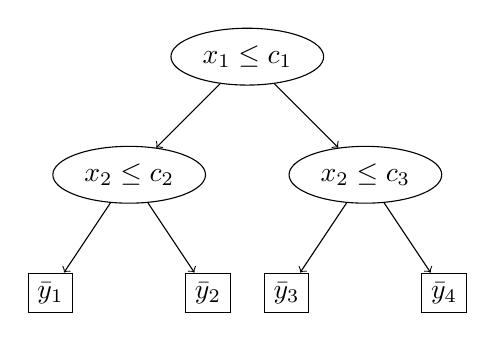
\begin{tikzpicture}[nodes={ellipse,draw}, ->]
      \tikzstyle{level 1}=[sibling distance=30mm]
      \tikzstyle{level 2}=[sibling distance=20mm] 
      \tikzstyle{every node}=[draw=black, ellipse, align=center]
      \draw node{$x_1 \leq c_1$}
      child{node{$x_2 \leq c_2$}
        child{node[rectangle] {$\bar{y}_1$}}
        child{node[rectangle] {$\bar{y}_2$}}
      }
      child{node{$x_2 \leq c_3$}
	    child{node[rectangle] {$\bar{y}_3$}}
	    child{node[rectangle] {$\bar{y}_4$}}
      }
      ;
    \end{tikzpicture}
  \end{minipage}
  \begin{minipage}{0,49\textwidth}
    \centering
    \begin{tikzpicture}[scale=0.7]
      \draw[->] (0,0) -- (7,0) node[right] {$x_1$}; 
      \draw[->] (0,0) -- (0,5) node[above] {$x_2$};
      \draw (3,0) -- (3,5);
      \draw (0,3) -- (3,3);
      \draw (3,4) -- (7,4);
      
      \draw (1.5, 1.8) node[below] {$\bar{y}_1$};
      \draw (1.5, 4) node[above] {$\bar{y}_2$};
      \draw (5, 2.4) node[below] {$\bar{y}_3$};
      \draw (5, 4.4) node[above] {$\bar{y}_4$};
      
      \draw (3, -0.05) -- (3, 0.05) node[below] {$c_1$};
      \draw (-0.05, 3) -- (0.05, 3) node[left] {$c_2$};
      \draw (-0.05, 4) -- (0.05, 4) node[left] {$c_3$};
    \end{tikzpicture}
  \end{minipage}
  \caption{A decision tree (to the left) partition an input space
    into disjoint regions (to the right), and associates each region
    with an output value.}
  \label{fig:decision-tree}
\end{figure}
%%%%%%%%%%%%%%%%%%%%%%%%%%%%%%%%%%%%%%%%%%%%%%%%%%%%%%%%%%%%%%%%%%%%%%%%%%%%%%%%
In general, decision rules in decision trees may be non-linear and multivariate. 
Although researchers have demonstrated that decision trees with 
non-linear~\shortcite{Irsoy12} and multivariate~\shortcite{WangF18} decision 
rules can be useful, state-of-the-art implementations of tree-based machine 
learning models normally only contain univariate and linear decision rules, 
e.g., the popular machine learning libraries scikit-learn~\shortcite{Pedregosa11},
XGBoost~\shortcite{Chen16}, and CatBoost~\shortcite{Prokhorenkova18}.
In this paper, we formalize the prediction function without explicitly stating 
decision rules.
%%%%%%%%%%%%%%%%%%%%%%%%%%%%%%%%%%%%%%%%%%%%%%%%%%%%%%%%%%%%%%%%%%%%%%%%%%%%%%%%
\begin{definition}[Decision Tree Prediction Function]
\label{def:decision-tree}
Let $X_1, \ldots, X_k$ be a partition of an $n$-dimensional input space, 
$\bar{y_1}, \ldots, \bar{y_k}$ values from an $m$-dimensional output space, 
and $T = \{(X_1, \bar{y_1}), \ldots, (X_k, \bar{y_k})\}$.
The prediction function for a decision tree may then be defined as
\begin{equation*}
  t(\bar{x}; T) = 
  \begin{cases} 
    \bar{y_1} & \text{if } \bar{x} \in X_{1}, \\
     &  \vdots\\
    \bar{y_k} & \text{if } \bar{x} \in X_{k}. \\
  \end{cases}
\end{equation*}
\end{definition}
%%%%%%%%%%%%%%%%%%%%%%%%%%%%%%%%%%%%%%%%%%%%%%%%%%%%%%%%%%%%%%%%%%%%%%%%%%%%%%%%
When decision trees only contain univariate and linear decision rules, the 
partitioned input space $X_1, \ldots, X_k$ forms adjacent
hyperrectangles (boxes), as exemplified by Figure~\ref{fig:decision-tree}.

A decision tree trained on a dataset with $n$ features may contain unreferenced
variables, i.e., the tree only considers a subset of its input variables during 
prediction. This is typically the case in high-dimensional applications, or 
when the training dataset contains statistically insignificant features. 
Since such input variables never affect predictions, they never appear in
minimal explanations. Consequently, we define the notion of \textit{variables
referenced by a tree}, which we later use in Section~\ref{sec:algos} to 
improve the runtime performance when computing minimal and minimum explanations.
%%%%%%%%%%%%%%%%%%%%%%%%%%%%%%%%%%%%%%%%%%%%%%%%%%%%%%%%%%%%%%%%%%%%%%%%%%%%%%%%
\begin{definition}[Variables Referenced by a Tree]
\label{def:var-ref-tree}
The variables referenced by a tree during predictions is a set of indices
$V_t \subseteq \{1, \ldots, n\}$, defined as the union of all the dimensions 
its decision rules operate in.
\end{definition}
For example, the decision tree illustrated in Figure~\ref{fig:decision-tree} 
operates on $x_1$ and $x_2$, in which case $V_t = \{1, 2\}$.
%%%%%%%%%%%%%%%%%%%%%%%%%%%%%%%%%%%%%%%%%%%%%%%%%%%%%%%%%%%%%%%%%%%%%%%%%%%%%%%%
\subsubsection{Tree Ensembles}
Decision trees are known to suffer from overfitting, i.e., the model becomes 
too specialized towards training data, and the prediction function generalizes 
poorly when confronted with previously unseen inputs. To counteract overfitting 
of decision trees, several types of tree ensembles have been proposed, e.g., 
random forests~\shortcite{Breiman01} and gradient boosting 
machines~\shortcite{Friedman01}. The different types of tree ensembles are 
normally distinguished by their learning algorithms, while their prediction
functions have similar structure.
%%%%%%%%%%%%%%%%%%%%%%%%%%%%%%%%%%%%%%%%%%%%%%%%%%%%%%%%%%%%%%%%%%%%%%%%%%%%%%%%
\begin{definition}[Tree Ensemble Prediction Function]
\label{def:tree-ensemble}
Let $F = (T_1, \ldots, T_b)$ be a tuple of $b \in \mathbb{Z}_{+}$ decision
trees (as defined by Definition~\ref{def:decision-tree}), all sharing the same
$n$-dimentional input space and $m$-dimentional output space. The prediction 
function for a tree ensemble may then be defined as
\begin{equation*}
  \label{eq:tree-ensemble}
  f(\bar{x}; F) = \sum_{T \in F} t(\bar{x}; T).
\end{equation*}
\end{definition}
When leaves in decision trees are associated with tuples of scalars, $f$ 
applies the addition operator element-wise.

Similar to a decision tree, an ensemble of trees may also only consider a 
subset of its input variables during prediction.
\begin{definition}[Variables Referenced by a Tree Ensemble]
\label{def:var-ref-ensemble}
The variables referenced by a tree ensemble during predictions is a set of indices
$V_f \subseteq \{1, \ldots, n\}$, defined as the union of all variables
referenced by the individual trees in the ensemble.
\end{definition}

%%%%%%%%%%%%%%%%%%%%%%%%%%%%%%%%%%%%%%%%%%%%%%%%%%%%%%%%%%%%%%%%%%%%%%%%%%%%%%%%
\subsubsection{Classification with Tree Ensembles}
\label{sec:classification}
By training tree ensembles to predict probabilities, they can be used as 
classifiers. Classifiers trained using XGBoost have tree leaves that are
associated with scalar values that are summed together in the logarithmic scale,
followed by a transformation to the domain of probabilities. For binary
classifications, the used transform function is the sigmoid function.
%%%%%%%%%%%%%%%%%%%%%%%%%%%%%%%%%%%%%%%%%%%%%%%%%%%%%%%%%%%%%%%%%%%%%%%%%%%%%%%%
\begin{definition}[Sigmoid Function]
\label{def:sigmoid}
The sigmoid function $p_{\sigma}$ is a function that transforms a real-valued 
input $z$ into an output value in the range $[0, 1]$, and is defined as
\begin{equation*}
  \label{eq:sigmoid}
  p_{\sigma}(z) = \frac{1}{1 + e^{-z}}.
\end{equation*}
\end{definition}
%%%%%%%%%%%%%%%%%%%%%%%%%%%%%%%%%%%%%%%%%%%%%%%%%%%%%%%%%%%%%%%%%%%%%%%%%%%%%%%%
With the sigmoid function defined, we can define the tree-based binary 
classifier.
\begin{definition}[Tree-based Binary Classifier]
\label{def:binary-classifier}
Let $F$ be a tree ensemble trained to predict the probability that a given
input tuple $\bar{x}$ maps to one of two classes. A binary classifier $f_{bin}$
that discriminates between the two classes may then be defined as
\begin{equation*}
  \label{eq:binary-classifier}
  f_{bin}(\bar{x}; F) = p_{\sigma}\big(f(\bar{x}; F)\big) > 0.5.
\end{equation*}
\end{definition}
%%%%%%%%%%%%%%%%%%%%%%%%%%%%%%%%%%%%%%%%%%%%%%%%%%%%%%%%%%%%%%%%%%%%%%%%%%%%%%%%
To capture statistical properties of multi-class systems involving three or 
more classes, some machine learning libraries associate tree leaves with 
tuples of probabilities~\shortcite<e.g.,>{Prokhorenkova18}, while others use
the \textit{one-vs-rest} classification paradigm~\shortcite<e.g.,>{Chen16}. 
Both of these approaches use the softmax function to transform values from 
the logarithmic domain to the domain of probabilities.
%%%%%%%%%%%%%%%%%%%%%%%%%%%%%%%%%%%%%%%%%%%%%%%%%%%%%%%%%%%%%%%%%%%%%%%%%%%%%%%%
\begin{definition}[Softmax Function]
\label{def:softmax}
The softmax function $p_s$ is a monotonic function that transforms a tuple of
real-valued inputs into an output tuple with elements in the range $[0, 1]$
such that those elements sum up to one, and is defined as
\begin{equation*}
  \label{eq:argmax}
  p_s(z_1, \ldots, z_m) = \frac{(e^{z_1}, \ldots, e^{z_m})}{\sum\limits_{i=1}^{m}z_i}.
\end{equation*}
\end{definition}
%%%%%%%%%%%%%%%%%%%%%%%%%%%%%%%%%%%%%%%%%%%%%%%%%%%%%%%%%%%%%%%%%%%%%%%%%%%%%%%%
This work focuses on classifiers trained using XGBoost, which implements the
\textit{one-vs-rest} paradigm for multi-class classification.
%%%%%%%%%%%%%%%%%%%%%%%%%%%%%%%%%%%%%%%%%%%%%%%%%%%%%%%%%%%%%%%%%%%%%%%%%%%%%%%%
\begin{definition}[Tree-based Multi-class Classifier]
\label{def:multi-classifier}
Let $C=(F_1,\ldots,F_m$) be a collection of tree ensembles such that the $i$-th 
tree ensemble $F_i$ is trained to predict the probability that a given instance
belongs to the $i$-th class. A multi-class classifier $f_{cls}$ that 
discriminates between the multiple classes may then be defined as
\begin{equation*}
  \label{eq:multiclass-classifier}
  f_{cls}(\bar{x}; C) = 
    \min\Big(\argmax_{\{1, \ldots, m\}}\Big(p_s\big(f(\bar{x}; F_1), 
                                                      \ldots, 
                                                      f(\bar{x}; F_m)
                                                 \big)
                                        \Big)
    \Big)
\end{equation*}
\end{definition}
%%%%%%%%%%%%%%%%%%%%%%%%%%%%%%%%%%%%%%%%%%%%%%%%%%%%%%%%%%%%%%%%%%%%%%%%%%%%%%%%
In principle, a multi-class classifier may predict that a given input belongs
to different classes with the exact same probability, and thus may cause the
argmax function to yield a set containing several classes. In these types of
situations, machine learning libraries typically return only the class with
the smallest index, being indifferent to the selected choice of class.
%%%%%%%%%%%%%%%%%%%%%%%%%%%%%%%%%%%%%%%%%%%%%%%%%%%%%%%%%%%%%%%%%%%%%%%%%%%%%%%%
\subsection{Abstract Interpretation of Computer Programs}
\label{sec:absint}
Abstract interpretation is a framework introduced to facilitate sound and 
efficient reasoning about programs being analyzed by a compiler~\shortcite{Cousot77}. 
The idea is to transform the source code of a program that computes values in a 
concrete domain into functions that operate in one or more abstract domains 
in which some analyses of interest are faster than in the corresponding concrete
domain, but potentially less precise. 

%%%%%%%%%%%%%%%%%%%%%%%%%%%%%%%%%%%%%%%%%%%%%%%%%%%%%%%%%%%%%%%%%%%%%%%%%%%%%%%%
For example, to initiate the analysis of a program running with floating-point 
numbers to work within the domain of intervals, an abstraction function 
$\alpha: \PFP \rightarrow \I$ is used to map a set of values from the 
floating-point domain $\FP$ to values from the interval domain $\I$. 
Analogously, a concretization function $\gamma: \I \rightarrow \PFP$ is used to
map an interval to a set of floating-point numbers. Abstraction and 
concretization mappings that operate on certain domains lead to a property 
called Galois connection that ensures sound reasoning with abstract 
interpretation~\shortcite{Cousot77}.
%%%%%%%%%%%%%%%%%%%%%%%%%%%%%%%%%%%%%%%%%%%%%%%%%%%%%%%%%%%%%%%%%%%%%%%%%%%%%%%%
\begin{definition}[Galois Connection]
\label{def:galois-connection}
Let $\alpha: \D \rightarrow \A$ and $\gamma: \A \rightarrow \PD$ be two 
monotone functions. A Galois connection $\PD \galois{\alpha}{\gamma} \A$ 
exist between the concrete domain $\D$ and the abstract domain $\A$ iff
\begin{gather*}\label{eq:galois-connection}
    \forall X \in \PD, X \subseteq \gamma(\alpha(X)), \\
    \forall \abs{x} \in \A, \abs{x} = \alpha(\gamma(\abs{x})).
  \end{gather*}
\end{definition}
%%%%%%%%%%%%%%%%%%%%%%%%%%%%%%%%%%%%%%%%%%%%%%%%%%%%%%%%%%%%%%%%%%%%%%%%%%%%%%%%
To perform the analysis, the program is interpreted in the abstract domain by
evaluating sequences of abstract values, operators, and transformers.
%%%%%%%%%%%%%%%%%%%%%%%%%%%%%%%%%%%%%%%%%%%%%%%%%%%%%%%%%%%%%%%%%%%%%%%%%%%%%%%%
\begin{definition}[Abstract Transformer]
\label{def:abstract-transformer}
An abstract transformer $\abs{f}: \A \rightarrow \A$ is an abstract counterpart
of a concrete function $f: \D \rightarrow \D$, but one that operates in the
abstract domain. 
\end{definition}
%%%%%%%%%%%%%%%%%%%%%%%%%%%%%%%%%%%%%%%%%%%%%%%%%%%%%%%%%%%%%%%%%%%%%%%%%%%%%%%%
When using abstract interpretation in a reasoning context, soundness can be 
ensured by proving that there exists a Galois connection between the concrete
and abstract domains, hence all computations performed in the abstract domain 
with the corresponding transformers are conservative.
%%%%%%%%%%%%%%%%%%%%%%%%%%%%%%%%%%%%%%%%%%%%%%%%%%%%%%%%%%%%%%%%%%%%%%%%%%%%%%%%
\begin{definition}[Conservative Transformer]
\label{def:conservative-transformation}
Let $\alpha: \PD \rightarrow \A$ be an abstraction function, 
and $\gamma: \A \rightarrow \PD$ a concretization function.
An abstract transformer $\abs{f}: \A \rightarrow \A$ is conservative with
respect to a concrete function $f: \D \rightarrow \D$ iff
\begin{equation*}
\label{eq:conservative-transformation}
\forall X \in \PD, \forall x \in X, f(x) \in \gamma(\abs{f}(\alpha(X))).
\end{equation*}
\end{definition}
%%%%%%%%%%%%%%%%%%%%%%%%%%%%%%%%%%%%%%%%%%%%%%%%%%%%%%%%%%%%%%%%%%%%%%%%%%%%%%%%
Abstract transformers for standard operators in concrete domains or sets
over such domains, e.g., addition and inclusion, can analogously be defined 
in a conservative manner. In this paper, we leverage an abstract interpreter 
that performs computations in the interval domain.
%%%%%%%%%%%%%%%%%%%%%%%%%%%%%%%%%%%%%%%%%%%%%%%%%%%%%%%%%%%%%%%%%%%%%%%%%%%%%%%%
\begin{definition}[Interval Domain]
\label{def:interval-domain}
The interval domain $\I$ contains abstract values $\abs{x}$ that capture sets 
of values from a concrete domain $\D$ using a range defined by a lower and upper
inclusive bound, i.e., $\abs{x} = [l,u]$, where $l, u \in \D, l \leq u$ are 
the lower and upper bound, respectively. Table~\ref{tbl:intdom} defines natural
abstraction and concretization functions, operators, and constants associated 
with the interval domain.
%%%%%%%%%%%%%%%%%%%%%%%%%%%%%%%%%%%%%%%%%%%%%%%%%%%%%%%%%%%%%%%%%%%%%%%%%%%%%%%%
\begin{table}[ht]
  \centering
  \begin{tabular}{ll}
    \hline
    \textbf{Name}       & \textbf{Definition} \\
    \hline
    Abstraction  & $\alpha(V) = [\min V, \max V]$ \\
    Concretization & $\gamma([v_1, v_2]) = \{v : v_1 \leq v \leq v_2\}$ \\
    Top        & $\top = \alpha(\D)$ \\
    Bottom     & $\bot = \alpha(\emptyset)$\\
    Addition   & $\abs{v} + \abs{u} = [v_1 + u_1, v_2 + u_2]$ \\
    Join       & $\abs{v} \sqcup \abs{u} = [\min(v_1, u_1), \max(v_2, u_2)]$ \\
    Meet       & $\abs{v} \sqcap \abs{u} = 
                     \begin{cases} 
                        \bot \text{ if } \max(v_1,u_1) > \min(v_2,u_2),\\
                        [\max(v_1, u_1), \min(v_2, u_2)] \text{ otherwise} \\
                     \end{cases}
                 $ \\
    Greater than & $\abs{v} > \abs{u} = 
                     \begin{cases} 
                       [0, 0] \text{ if } \min(u_1, u_2) > \max(v_1, v_2), \\
                       [1, 1] \text{ if } \min(v_1, v_2) > \max(u_1, u_2), \\
                       [0, 1] \text{ otherwise}\\
                     \end{cases}
                 $ \\
    \hline
  \end{tabular}
  \caption{Abstract interpretation in the interval domain $\I$ over 
           values from the concrete domain $\D$, where $V \subseteq \D$, 
           $v, v_1, v_2, u_1, u_2 \in \D$, and
           $\abs{v} = [v_1, v_2], \abs{u} = [u_1, u_2] \in \I$.}
  \label{tbl:intdom}
\end{table}
\end{definition}
%%%%%%%%%%%%%%%%%%%%%%%%%%%%%%%%%%%%%%%%%%%%%%%%%%%%%%%%%%%%%%%%%%%%%%%%%%%%%%%%
Abstract interpretation of programs with multiple variables in the interval 
domain form hyperrectangles, in which case the domain is often referred to as 
the Box domain.

%%%%%%%%%%%%%%%%%%%%%%%%%%%%%%%%%%%%%%%%%%%%%%%%%%%%%%%%%%%%%%%%%%%%%%%%%%%%%%%%
\section{Related Works}
\label{sec:related-works}
The use of formal methods to prove correctness of explanations for predictions
made by machine learning systems has been promoted fairly recently.
\shortciteA{Shih18}~compute minimal explanations for classifications made by 
Bayesian networks. By compiling the prediction function of Bayesian networks 
into an ordered (non-binary) decision diagram, they are able to compute 
explanations efficiently. The computational challenges instead lie in the 
compilation of Bayesian networks into decision diagrams, rather than the 
computation of explanations~\shortcite{Shih19}.

%%%%%%%%%%%%%%%%%%%%%%%%%%%%%%%%%%%%%%%%%%%%%%%%%%%%%%%%%%%%%%%%%%%%%%%%%%%%%%%%
\shortciteA{Ignatiev19} demonstrate that off-the-shelf constraint solvers, 
e.g., SMT and MILP solvers, can be used to minimize explanations if the
prediction function can be represented within the used reasoning engine. They
assess scalability in terms of time taken to compute explanations for
predictions made by several neural networks trained on different datasets. 
Through experiments, they demonstrate that a state-of-the-art MILP solver 
typically outperforms most SMT solvers, and that computing explanations for 
models trained on high-dimensional inputs is significantly more demanding 
than low-dimensional problems. Compared to that work, we develop a framework
to embed a reasoning engine that is tailored specifically for tree ensembles
to achieve improved runtime performance.

%%%%%%%%%%%%%%%%%%%%%%%%%%%%%%%%%%%%%%%%%%%%%%%%%%%%%%%%%%%%%%%%%%%%%%%%%%%%%%%%
\shortciteA{La21} also compute explanations for neural networks, but use
reasoning engines designed specifically for the analysis of neural networks. 
They compare two different algorithms for computing a minimum explanation, 
both based on prior work, but with several novel algorithmic improvements. 
One algorithm is based on a branch-and-bound approach~\shortcite{Dillig12}, 
and the other is based on hitting sets~\shortcite{Ignatiev16}. 
In their Appendix\footnote{Available at https://arxiv.org/pdf/2105.03640.pdf}, 
they demonstrate that their improved branch-and-bound approach is typically 
faster than the hitting sets approach. In this work, we use a similar
branch-and-bound approach to compute minimum explanations, but for 
predictions made by tree ensembles, a model which has demonstrated greater
predictive capabilities than neural networks in several practical
applications~\shortcite{Shwartz22}.

%%%%%%%%%%%%%%%%%%%%%%%%%%%%%%%%%%%%%%%%%%%%%%%%%%%%%%%%%%%%%%%%%%%%%%%%%%%%%%%%
\shortciteA{Izza21} use a SAT solver to compute minimal explanations for
non-trivial random forests (100 trees with depths ranging from three to eight).
They also show that this computational problem is DP-complete, i.e.,
the class of computations involving both NP-complete and coNP-complete 
sub-problems.
Around the same time, \shortciteA{Boumazouza21} also used a SAT solver to 
compute minimal explanations for random forests, but with a different encoding.
They argue for the use of random forests as surrogates for models for which
no direct SAT-encoding exists.
%%%%%%%%%%%%%%%%%%%%%%%%%%%%%%%%%%%%%%%%%%%%%%%%%%%%%%%%%%%%%%%%%%%%%%%%%%%%%%%%
\shortciteA{Audemard22} present the notion of majority reasons for the 
purpose of explaining predictions made by random forests. These explanations
are significantly less computationally demanding to compute than minimal
explanations, at the potential expense of some verbosity. They also show%
\footnote{Proof available at https://arxiv.org/pdf/2108.05276.pdf}
that the problem of computing a minimum explanation is $\Sigma_2^p$-complete,
i.e., NP-complete with a coNP oracle.
In this work, we aim at reducing the runtime needed to compute explanations, 
but without compromising on verbosity. 

%%%%%%%%%%%%%%%%%%%%%%%%%%%%%%%%%%%%%%%%%%%%%%%%%%%%%%%%%%%%%%%%%%%%%%%%%%%%%%%%
\shortciteA{Ignatiev22} propose an approach that uses a MaxSAT-based oracle when 
computing minimal explanations of predictions made by tree ensembles. The 
approach is based on the application of the deletion 
filter~\shortcite{Chinneck91}, which is evaluated on gradient boosting machines
trained on 21 different datasets. They formulate the hard part of the MaxSAT 
encoding as a CNF formula, where intervals are represented by auxiliary Boolean
variables, while the validity of an explanation is encoded as weighted soft 
clauses that can be optimized to find a minimal explanation.
%%%%%%%%%%%%%%%%%%%%%%%%%%%%%%%%%%%%%%%%%%%%%%%%%%%%%%%%%%%%%%%%%%%%%%%%%%%%%%%%
In this work, we also use a deletion filter, but with an oracle based on 
abstract interpretation which is designed specifically for tree ensembles. 
Compared to the MaxSAT approach, our oracle operates on an implicit DNF encoding
of relaxed constraints that captures input-output relations derived from a tree 
ensemble. The relaxed constraints are captured by abstract values from the 
interval domain, which are enumerated and iteratively tightened in an 
abstraction-refinement loop~\shortcite{Tornblom19}. Furthermore, we tackle 
the computation of minimum explanations, and complete enumeration of all 
minimal explanations.

%%%%%%%%%%%%%%%%%%%%%%%%%%%%%%%%%%%%%%%%%%%%%%%%%%%%%%%%%%%%%%%%%%%%%%%%%%%%%%%%
The MARCO algorithm~\shortcite{Liffiton16} has been applied to a broad range
of problems, including for enumerating minimal explanations of prediction made
by decision lists~\shortcite{Ignatiev21} and monotonic
classifiers~\shortcite{Marques21}. Compared to those works, we demonstrate 
that the pairing of the MARCO algorithm with an oracle formalized in the 
abstract interpretation framework can make the enumeration of all minimal 
explanations for several predictions made by non-trivial tree ensembles 
tractable. We also adapt MARCO for computing explanations that are minimum
with respect to the weighted sum $g(I; W) = \sum_{i \in I}w_i$, where 
$I \subseteq \{1, \ldots, n\}$ and $W = (w_1, \ldots, w_n) \in \R_{\ge 0}^n$,
demonstrating a speedup factor of two compared to the enumeration of all
minimal explanations.

%%%%%%%%%%%%%%%%%%%%%%%%%%%%%%%%%%%%%%%%%%%%%%%%%%%%%%%%%%%%%%%%%%%%%%%%%%%%%%%%
A very recent work~\shortcite{Izza22} tackles the problem of removing redundancy
in explanations for predictions made by decision trees. Our work applies 
to ensembles of decision trees, and aims at computing explanations that are 
minimum with respect to a domain-specific cost function, motivated by the 
comprehensive field guide on explainability by~\shortciteA{Ras22}.

%%%%%%%%%%%%%%%%%%%%%%%%%%%%%%%%%%%%%%%%%%%%%%%%%%%%%%%%%%%%%%%%%%%%%%%%%%%%%%%%
\section{Constructing an Oracle based on Abstract Interpretation}
\label{sec:oracle}
In this section, we formalize the inner workings of a valid explanation oracle 
(see Definition~\ref{def:valid-exp-oracle}), designed specifically for tree 
ensembles using the concept of abstract interpretation. First, we define 
abstract transformers, which are necessary building blocks when constructing 
the oracle (Section~\ref{sec:abs-transformers}). Next, we define the abstract 
valid explanation oracle, together with an abstraction-refinement approach 
which ensures that abstractions that are too conservative are refined into 
more precise ones (Section~\ref{sec:abs-valid-oracle-def}). Finally, we 
assemble the building blocks into a sound and complete valid explanation 
oracle (Section~\ref{sec:abs-valid-oracle-construction}).

Since the input dimension of a tree ensemble is typically different from 
its output dimension, we sometimes subscript abstraction and concretization 
functions to indicate which dimensionality they operate on, e.g., 
$\powerset{\D^n} \galois{\alpha_n}{\gamma_n} \A^n$, and we denote 
tuples of abstract values using capital letters, e.g., 
$\absvec{x} = (\abs{x}_1, \ldots, \abs{x}_n)$. Subscripted abstraction and 
concretization functions apply the corresponding non-subscripted function 
element-wise as follows.
\begin{equation*}
  \label{eq:subscript-notation}
  \begin{aligned}
    \absvec{x} &= \alpha_n(\{\bar{x}\}) \\
    &= \alpha_n(\{(x_1, \ldots, x_n)\}) \\ 
    &= (\alpha(\{x_1\}), \ldots, \alpha(\{x_n\})) \\
    &= (\abs{x}_1, \ldots, \abs{x}_n),
  \end{aligned}
\end{equation*}
where $\bar{x} \in \D^n$.
%%%%%%%%%%%%%%%%%%%%%%%%%%%%%%%%%%%%%%%%%%%%%%%%%%%%%%%%%%%%%%%%%%%%%%%%%%%%%%%%
\subsection{Abstract Transformers}
\label{sec:abs-transformers}
We begin by defining the abstract transformers we later use to interpret 
tree-based classifiers; the decision tree transformer, the ensemble transformer, 
and the sigmoid transformer.

%%%%%%%%%%%%%%%%%%%%%%%%%%%%%%%%%%%%%%%%%%%%%%%%%%%%%%%%%%%%%%%%%%%%%%%%%%%%%%%%
\begin{definition}[Tree Transformer]
\label{def:tree-transformer}
Let $T = \{(X_1,\bar{y}_1), \ldots, (X_k,\bar{y}_k)\}$ be a decision tree as 
defined by Definition~\ref{def:decision-tree}, and $\alpha$ an abstraction 
function. The decision tree transformer $\abs{t}$ is then defined as
\begin{equation*}
  \label{eq:tree-transformer}
  \abs{t}(\absvec{x}; T) = \alpha_m(\{\bar{y}_i : (X_i,\bar{y}_i) \in T, 
                           \absvec{x} \sqcap \alpha_n(X_i) \ne \bot\}).
\end{equation*}
\end{definition}
%%%%%%%%%%%%%%%%%%%%%%%%%%%%%%%%%%%%%%%%%%%%%%%%%%%%%%%%%%%%%%%%%%%%%%%%%%%%%%%%
Given an abstract input tuple $\absvec{x}$, the transformer enumerates all pairs
$(X_i, \bar{y}_i)$ in the decision tree $T$, and checks whether there are 
overlapping values between the abstraction of the input region $X_i$ and the 
values captured by $\absvec{x}$, in which case $\bar{y}_i$ is included in 
the applied output abstraction.
%%%%%%%%%%%%%%%%%%%%%%%%%%%%%%%%%%%%%%%%%%%%%%%%%%%%%%%%%%%%%%%%%%%%%%%%%%%%%%%%
\begin{lemma}[Conservative Tree Transformer]
\label{lemma:tree}
The transformer $\abs{t}$ as defined by Definition~\ref{def:tree-transformer}
is conservative with respect to the prediction function $t$ as defined by
Definition~\ref{def:decision-tree} if the abstraction function $\alpha$ forms
a Galois connection with the used concretization function $\gamma$, i.e., that 
$\forall \bar{x} \in \D^n, t(\bar{x}; T) \in \gamma_m(\abs{t}(\alpha_n(\{\bar{x}\})); T)$,
where $n$ and $m$ are the input and output dimensions, respectively.
\end{lemma}
%%%%%%%%%%%%%%%%%%%%%%%%%%%%%%%%%%%%%%%%%%%%%%%%%%%%%%%%%%%%%%%%%%%%%%%%%%%%%%%%
\begin{proof}
Let $\bar{x} \in \D^n$ be an arbitrary value from the concrete input domain, 
$(X, \bar{y}) \in T$ such that $\bar{x} \in X$, and thus $t(\bar{x}) = \bar{y}$. 
According to Definition~\ref{def:conservative-transformation}, the transformer 
$\abs{t}$ is conservative iff $\bar{y} \in \gamma_m(\abs{t}(\alpha_n(\{\bar{x}\}); T))$. 
By expanding $\abs{t}$ and using the fact that $t$ maps $\bar{x}$ to $\bar{y}$, 
we obtain
\begin{equation*}
\begin{split}
\bar{y} \in\text{ }& \gamma_m(\abs{t}(\alpha_n(\{\bar{x}\}); T)) = \\
                     & \gamma_m(\alpha_m(\{\bar{y}_i : (X_i,\bar{y}_i) \in T, 
                                \alpha_n(\{\bar{x}\}) \sqcap \alpha_n(X_i) \ne \bot\})) = \\
                     & \gamma_m(\alpha_m(\{\bar{y}\}))
\end{split}
\end{equation*} 

which holds when $\alpha$ and $\gamma$ form a Galois connection between the 
domains $\D$ and $\A$.
\end{proof}
%%%%%%%%%%%%%%%%%%%%%%%%%%%%%%%%%%%%%%%%%%%%%%%%%%%%%%%%%%%%%%%%%%%%%%%%%%%%%%%%
Next, we define the ensemble transformer as the sum over a set of tree
transformations.
\begin{definition}[Ensemble Transformer]
\label{def:ensemble-transformer}
Let $F = (T_1, \ldots, T_B)$ be a tree ensemble as defined by
Definition~\ref{def:tree-ensemble}. The tree ensemble transformer is then 
defined as
\begin{equation*}
    \abs{f}(\absvec{x}; F) = \sum\limits_{i=1}^{B} \abs{t}(\absvec{x}; T_i).
\end{equation*}
\end{definition}
%%%%%%%%%%%%%%%%%%%%%%%%%%%%%%%%%%%%%%%%%%%%%%%%%%%%%%%%%%%%%%%%%%%%%%%%%%%%%%%
\begin{lemma}[Conservative Ensemble Transformer]
\label{lemma:ensemble}
The transformer $\abs{f}$ as defined by Definition~\ref{def:ensemble-transformer}
is conservative with respect to the prediction function $f$ as defined by
Definition~\ref{def:tree-ensemble} if $\powerset{\D}\galois{\alpha}{\gamma}\A$ 
form a Galois connection, and the addition operator in the used abstract domain 
is conservative.
\end{lemma}
%%%%%%%%%%%%%%%%%%%%%%%%%%%%%%%%%%%%%%%%%%%%%%%%%%%%%%%%%%%%%%%%%%%%%%%%%%%%%%%%
\begin{proof}
By using Lemma~\ref{lemma:tree} with the assumption on the abstract transformer
for the addition operator, all individual transformations performed by $\abs{f}$
are conservative, hence $\abs{f}$ is conservative.
\end{proof}
For gradient boosting machines trained on binary classification problems, we 
post-process the sum of trees with an abstract counterpart to the sigmoid 
function (Definition~\ref{def:sigmoid}).
%%%%%%%%%%%%%%%%%%%%%%%%%%%%%%%%%%%%%%%%%%%%%%%%%%%%%%%%%%%%%%%%%%%%%%%%%%%%%%%%
\begin{definition}[Sigmoid Transformer]
Let $p_{\sigma}$ be the concrete sigmoid function (as defined by 
Definition~\ref{def:sigmoid}). The abstract sigmoid transformer 
$\abs{p}_{\sigma}$ is then defined as
\label{def:sigmoid-transformer}
\begin{equation*}
\abs{p}_{\sigma}(\abs{z}) = \alpha
\Big(\big\{
  p_{\sigma}(\min(\abs{z})), 
  \ldots,
  p_{\sigma}(\max(\abs{z}))
\big\}\Big)
\end{equation*}
\end{definition}
%%%%%%%%%%%%%%%%%%%%%%%%%%%%%%%%%%%%%%%%%%%%%%%%%%%%%%%%%%%%%%%%%%%%%%%%%%%%%%%%
\begin{lemma}[Conservative Sigmoid Transformer]
\label{lemma:sigmoid}
The transformer $\abs{p}_{\sigma}$ as defined by 
Definition~\ref{def:sigmoid-transformer} is conservative with respect to the 
concrete sigmoid function as defined by Definition~\ref{def:sigmoid}.
\end{lemma}
%%%%%%%%%%%%%%%%%%%%%%%%%%%%%%%%%%%%%%%%%%%%%%%%%%%%%%%%%%%%%%%%%%%%%%%%%%%%%%%%
\begin{proof}
Let $Z \subseteq \D$ be an arbitrary subset of the concrete domain, $z \in Z$ 
an arbitrary element from that subset, 
$P: \{p_{\sigma}(\min(Z)), \ldots, p_{\sigma}(\max(Z))\}$, and
$p'_{\sigma}(z) = p_{\sigma}(z)(1 - p_{\sigma}(z))$ the derivative of $p_{\sigma}$.
Since $p'_{\sigma}$ is non-negative and thus the successive applications of 
$p_{\sigma}$ yield values that are monotonically increasing, we know that 
$p_{\sigma}(z) \in P$.
Furthermore, according to
Definition~\ref{def:conservative-transformation}, we know that the transformer
$\abs{p}_{\sigma}$ is conservative iff 
$p_{\sigma}(z) \in \gamma(\abs{p}_{\sigma}(\alpha(Z)))$.
By carefully applying $\alpha$ and $\gamma$ to appropriate terms in $P$, we obtain
\begin{equation*}
\begin{split}
p_{\sigma}(z)\in\text{ }& \{p_{\sigma}(\min(Z)), \ldots, p_{\sigma}(\max(Z))\} \subseteq \\
                  & \gamma(\alpha(\{p_{\sigma}(\min(Z)), \ldots, p_{\sigma}(\max(Z))\})) \subseteq \\
                  & \gamma(\alpha(\{p_{\sigma}(\min(\alpha(Z))), \ldots, p_{\sigma}(\max(\alpha(Z)))\})) = \\
                  & \gamma(\abs{p}_{\sigma}(\alpha(Z))),
\end{split}
\end{equation*} 
hence $\abs{p}_{\sigma}$ is conservative with respect to $p_{\sigma}$.
\end{proof}

%%%%%%%%%%%%%%%%%%%%%%%%%%%%%%%%%%%%%%%%%%%%%%%%%%%%%%%%%%%%%%%%%%%%%%%%%%%%%%%%
With the basic building blocks of tree-based classifiers formalized as 
abstract transformers, we can now define an abstract counter-part to the
binary classifier $f_{bin}$ introduced in Section~\ref{sec:classification}.
%%%%%%%%%%%%%%%%%%%%%%%%%%%%%%%%%%%%%%%%%%%%%%%%%%%%%%%%%%%%%%%%%%%%%%%%%%%%%%%%
\begin{definition}[Abstract Binary Classifier]
\label{def:abs-bin-classifier}
Let $F$ be a tree ensemble as defined by Definition~\ref{def:binary-classifier}. 
The abstract binary classifier $\abs{f}_{bin}$ is then defined as
\begin{equation*}
    \abs{f}_{bin}(\absvec{x}; F) = \abs{p}_{\sigma}(\abs{f}(\absvec{x}; F)) > \alpha(\{0.5\}).
\end{equation*}
\end{definition}
%%%%%%%%%%%%%%%%%%%%%%%%%%%%%%%%%%%%%%%%%%%%%%%%%%%%%%%%%%%%%%%%%%%%%%%%%%%%%%%%
\begin{lemma}
\label{lemma:bin-classifier}
The abstract binary classifier $\abs{f}_{bin}$ is conservative with respect
to the concrete binary classifier $f_{bin}$ as defined by 
Definition~\ref{def:binary-classifier} if the abstract transformer for the 
concrete operator $>$ is conservative.
\end{lemma}
%%%%%%%%%%%%%%%%%%%%%%%%%%%%%%%%%%%%%%%%%%%%%%%%%%%%%%%%%%%%%%%%%%%%%%%%%%%%%%%%
\begin{proof}
By using Lemma~\ref{lemma:ensemble}~and~\ref{lemma:sigmoid} together with the 
assumption on the abstract transformer for $>$, all individual transformations
performed by $\abs{f}_{bin}$ are conservative, hence $\abs{f}_{bin}$ is 
conservative.
\end{proof}

%%%%%%%%%%%%%%%%%%%%%%%%%%%%%%%%%%%%%%%%%%%%%%%%%%%%%%%%%%%%%%%%%%%%%%%%%%%%%%%%
\subsection{Abstract Valid Explanation Oracle}
\label{sec:abs-valid-oracle-def}
We now move on to define a valid explanation oracle for binary classifications
that operates in an abstract domain. 
%%%%%%%%%%%%%%%%%%%%%%%%%%%%%%%%%%%%%%%%%%%%%%%%%%%%%%%%%%%%%%%%%%%%%%%%%%%%%%%%
\begin{definition}[Abstract Valid Explanation Oracle for Binary Classifications]
\label{def:abs-expl-oracle}
Let $p: f_{bin}(c_1, \ldots, c_n; F) \mapsto d$ be a prediction, 
$S \subseteq \{1, \ldots, n\}$ a set with elements that encode the 
absence of variables with given indices in an explanation (as defined
by Definition~\ref{def:valid-exp-oracle}), and 
$\absvec{X} = (\abs{x}_1, \ldots, \abs{x}_n)$ an abstract input tuple that
captures all possible combinations of assignments to those absent variables, 
where the $i$-th element in $\absvec{X}$ is defined as
\begin{equation*}
  \abs{x}_i = 
  \begin{cases} 
    \top & \text{if } i \in S, \\
    \alpha({\{c_i\}}) & \text{otherwise}.
  \end{cases}
\end{equation*}
%%%%%%%%%%%%%%%%%%%%%%%%%%%%%%%%%%%%%%%%%%%%%%%%%%%%%%%%%%%%%%%%%%%%%%%%%%%%%%%%
An abstract valid explanation oracle $v_{bin}$ for binary classifications may 
then be defined as
\begin{equation*}
  v_{bin}(\absvec{X}, d; F) = 
  \begin{cases} 
    Pass & \text{if } \{d\} = \gamma(\abs{f}_{bin}(\absvec{X}; F)), \\
    Fail & \text{if } d \not\in \gamma(\abs{f}_{bin}(\absvec{X}; F)), \\
    Unsure & \text{otherwise}.
  \end{cases}
\end{equation*}
\end{definition}
%%%%%%%%%%%%%%%%%%%%%%%%%%%%%%%%%%%%%%%%%%%%%%%%%%%%%%%%%%%%%%%%%%%%%%%%%%%%%%%%
Similarly, an oracle $v_{cls}$ for predictions made by a multi-class classifier
$f_{cls}$ may be defined by replacing occurrences of $\abs{f}_{bin}$ in 
Definition~\ref{def:abs-expl-oracle} with $\abs{f}_{cls}$.
%%%%%%%%%%%%%%%%%%%%%%%%%%%%%%%%%%%%%%%%%%%%%%%%%%%%%%%%%%%%%%%%%%%%%%%%%%%%%%%%
\begin{theorem}[Soundness]
\label{theo:sound}
Given an explanation (as used within Definition~\ref{def:abs-expl-oracle}),
the abstract explanation oracle $v_{bin}$ that uses the conservative 
transformer $\abs{f}_{bin}$ is sound, i.e., whenever $v_{bin}$ returns 
$Pass$, the explanation is valid, and whenever $v_{bin}$ returns $Fail$, 
it is not valid.
\end{theorem}
%%%%%%%%%%%%%%%%%%%%%%%%%%%%%%%%%%%%%%%%%%%%%%%%%%%%%%%%%%%%%%%%%%%%%%%%%%%%%%%%
\begin{proof}
Since $\absvec{x}$ captures all possible combinations of assignments to the
absent variables (as defined in Definition~\ref{def:abs-expl-oracle}), and
$\abs{f}_{bin}$ is conservative (according to Lemma~\ref{lemma:bin-classifier}), 
we know that when $d \not\in \gamma(\abs{f}_{bin}(\absvec{x}; F))$, the given
explanation is not valid, which is the only case where $v_{bin}$ returns $Fail$.
If all input points captured by $\abs{X}$ are mapped by $f_{bin}$ to $d$, 
i.e., $\{d\} = \gamma(\abs{f}_{bin}(\absvec{x}; F))$, the explanation is valid,
which is the only case where $v_{bin}$ returns $Pass$. Consequently, $v_{bin}$ 
is sound.
\end{proof}

%%%%%%%%%%%%%%%%%%%%%%%%%%%%%%%%%%%%%%%%%%%%%%%%%%%%%%%%%%%%%%%%%%%%%%%%%%%%%%%%
In general, abstract interpretation is not complete, i.e., abstract transformers
may yield abstractions that are too conservative in order to provide conclusive
query responses when used in a reasoning engine, e.g., when our oracle in 
Definition~\ref{def:abs-expl-oracle} returns $Unsure$. In our case where tree 
ensembles only contain univariate and linear decision rules, however, there
exists algorithms designed specifically for abstract interpretation of tree
ensembles that refine abstractions that are too conservative into several
more concise ones, eventually leading to precise 
abstractions~\shortcite{Tornblom19,Ranzato20}. 
In this work, we leverage one of these algorithms, implemented in the tool 
suite VoTE~\shortcite{Tornblom19}, to construct an oracle that is both sound
and complete. VoTE has demonstrated great performance in terms of runtime and
memory usage~\shortcite{Tornblom21}, and provides a modular property checking 
interface realized as a recursive higher-order function. More specifically, 
VoTE accepts three parameters as input; a tree ensemble $F$, a tuple of 
intervals $\absvec{x} \in \I^n$ with $\bot \not\in \absvec{x}$, and a 
property checker $pc: \I^n \times \I^m \rightarrow \{Pass,Fail,Unsure\}$, as 
formalized by Algorithm~\ref{algo:VoTE}. The algorithm also accepts an 
auxiliary parameter $R \subseteq F$ that keeps track of refinement steps
during recursion, and is initialized to the empty set.

%%%%%%%%%%%%%%%%%%%%%%%%%%%%%%%%%%%%%%%%%%%%%%%%%%%%%%%%%%%%%%%%%%%%%%%%%%%%%%%%
\begin{algorithm}[ht]
  \caption{The abstraction-refinement algorithm implemented in VoTE, where
           $F$ is a tree ensemble, $\absvec{x}$ a tuple of intervals that capture
           points in the input domain, $pc$ a property checker, and $R$ a
           state-tracking auxiliary parameter initialized to $\emptyset$.}
  \label{algo:VoTE}
  \begin{algorithmic}[1]
    \Function{VoTE}{$F, \absvec{x}, pc, R=\emptyset$}
      \Let{$o$}{$pc(\absvec{x}, \abs{f}(\absvec{x}; F))$}
      \Comment{Compute outcome of property checker}
      \If{$o \ne Unsure$}
        \State \Return $o$
        \Comment{Property checker is conclusive with this abstraction}
      \ElsIf{$R = F$}
        \State \Return $o$
        \Comment{No more refinements necessary}
      \Else
        \State {$T \in F \backslash R$}
        \Comment{Select a tree not in $R$}
        \ForEach{$(X_i, \bar{y}_i) \in T$}
          \Comment{Enumerate leaves in the selected tree}
          \Let{$\absvec{x}_i$}{$\absvec{x} \sqcap \alpha_n(X_i)$}
          \Comment{Refine abstraction}
          \Let{$o$}{\Call{VoTE}{$F, \absvec{x}_i, pc, R \cup \{T\}$}}
          \Comment{Recursively check the refined abstraction}
          \If{$o \ne Pass$}
            \State \Return $o$
            \Comment{Stop enumerating if outcome is $Fail$ or $Unsure$}
          \EndIf
        \EndForEach
        \State \Return $Pass$
        \Comment{Property is satisfied for all inputs captured by $\absvec{x}$}
      \EndIf
    \EndFunction
  \end{algorithmic}
\end{algorithm}

%%%%%%%%%%%%%%%%%%%%%%%%%%%%%%%%%%%%%%%%%%%%%%%%%%%%%%%%%%%%%%%%%%%%%%%%%%%%%%%%
The algorithm starts by computing a conservative output approximation 
$\abs{f}(\absvec{x}; F)$, which is then checked by the given property checker 
$pc$ (line 2). If the property checker is conclusive, or if there are no more
refinements necessary (see the following Lemma~\ref{lemma:precise} and its 
proof why this is the case when $R = F$), the outcome of $pc$ is returned 
(lines 3--6). Otherwise, the algorithm picks an arbitrary tree $T$ from the 
ensemble $F$ that has not been picked before (line 8), and refines $\absvec{x}$ 
into a partition with abstract input tuples $\absvec{x}_1, \ldots, \absvec{x}_k$
(lines 9--15). For each refined abstraction $\absvec{x}_i$, the algorithm is
invoked recursively (line 11). Whenever a recursive invocation yields an 
outcome that does not guarantee satisfaction with the property checked by $pc$, 
i.e., whenever $pc$ returns $Fail$ or $Unsure$, the computed outcome is 
returned. When the tree ensemble satisfies the checked property for all input
values captured by $\absvec{x}$, the algorithm returns $Pass$ (line 16).

%%%%%%%%%%%%%%%%%%%%%%%%%%%%%%%%%%%%%%%%%%%%%%%%%%%%%%%%%%%%%%%%%%%%%%%%%%%%%%%%
\begin{lemma}[Precise Abstraction Refinement]
\label{lemma:precise}
Given a tuple of abstractions $\absvec{x}$ with $\bot \not\in \absvec{X}$,
and a property checker $pc$ that always returns $Unsure$, 
Algorithm~\ref{algo:VoTE} refines $\absvec{x}$ into a partition with more 
concise abstract input tuples $\absvec{x}_1, \ldots, \absvec{x}_k$, which 
eventually leads to precise output abstractions, i.e.,
$\forall i \in \{1, \ldots, k\}, |\gamma(\abs{f}(\absvec{x}_i; F))| = 1$.
\end{lemma}
\begin{proof}
%%%%%%%%%%%%%%%%%%%%%%%%%%%%%%%%%%%%%%%%%%%%%%%%%%%%%%%%%%%%%%%%%%%%%%%%%%%%%%%%
In each recursive step, the algorithm picks a tree $T$, and computes abstract
input tuples $\absvec{x}_1, \ldots, \absvec{x}_k$ such that the tree transformer
$\abs{t}$ yields a precise output abstractions for that particular tree, i.e., 
$\forall i \in \{1, \ldots, k\}, |\gamma_m(\abs{t}(\absvec{x}_i; T))| = 1$.
When $F=R$, all trees in the ensemble have gone through a refinement step, hence
$\forall T \in F, \forall i \in \{1, \ldots, k\}, |\gamma_m(\abs{t}(\absvec{x}_i; T))| = 1$.
In these cases, the summation operator in $\abs{f}$ transforms abstract values
that capture a single point in the output space, hence the total sum is also 
an abstraction of a single point, i.e.
$\forall i \in \{1, \ldots, k\}, |\gamma_m(\abs{f}(\absvec{x}_i); F)| = 1$.
\end{proof}

%%%%%%%%%%%%%%%%%%%%%%%%%%%%%%%%%%%%%%%%%%%%%%%%%%%%%%%%%%%%%%%%%%%%%%%%%%%%%%%%
\subsection{The Construction of a Valid Explanation Oracle}
\label{sec:abs-valid-oracle-construction}
Recall the problem we are tackling in this section, i.e., given a prediction
$p$ and an explanation $E$, determine if $E$ is valid with respect to $p$
(Definition~\ref{def:valid-exp}). Here, we focus on binary classifications, but 
our approach can be extended to the multi-class classifications, as formalized 
in Appendix~\ref{sec:sup-algos}. In the case of binary classification, the 
approach is formalized as Algorithm~\ref{algo:oracle}, which takes as input a tree 
ensemble $F$, a tuple $\absvec{X}$ of abstract input values constructed from the
given explanation $E$ according to Definition~\ref{def:abs-expl-oracle}, and the 
predicted label $d$. The algorithm returns $True$ if all input values captured
by $\absvec{X}$ are mapped to the label $d$ by the classifier $f_{bin}$, in 
which case $E$ is valid with respect to $p$. Otherwise, there is some input 
value $\bar{x}$ captured by $\absvec{X}$ such that $f_{bin}(\bar{x}) \ne d$, 
in which case $E$ is not valid with respect to $p$.

%%%%%%%%%%%%%%%%%%%%%%%%%%%%%%%%%%%%%%%%%%%%%%%%%%%%%%%%%%%%%%%%%%%%%%%%%%%%%%%%
\begin{algorithm}
  \caption{A valid explanation oracle that checks if the tree ensemble $F$ 
           maps all points captured by the abstract input tuple 
           $\absvec{x} = (\abs{x}_1, \ldots, \abs{x}_n)$ to the label 
           $d \in \{0, 1\}$.}
  \label{algo:oracle}
  \begin{algorithmic}[1]
    \Function{Is\_Valid}{$F, \absvec{x}, d$}
      \Function{$pc$}{$\absvec{x}_p, \abs{y}_p$}
      \Comment{Define a property checker with a closure that binds $d$}
        \Let{$D$}{$\gamma\big(\abs{p}_{\sigma}(\abs{y}_p) < \alpha(\{0.5\})\big)$}
        \Comment{Equivalent to $\gamma\big(\abs{f}_{bin}(\absvec{x}; F)\big)$ since $\abs{y} = \abs{f}(\absvec{x}; F)$}
        \If{$|D| \ne 1$}
          \State \Return $Unsure$
          \Comment{Predicted output may be either $0$ or $1$}
        \ElsIf{$d \in D$}
          \State \Return $Pass$
          \Comment{Explanation is valid}
        \EndIf
        \State \Return $Fail$
        \Comment{Explanation is not valid}
      \EndFunction
      \State \Return \Call{VoTE}{$F, \absvec{x}, pc$} = $Pass$
      \Comment{Return $True$ if VoTE returns $Pass$}
    \EndFunction
  \end{algorithmic}
\end{algorithm}

%%%%%%%%%%%%%%%%%%%%%%%%%%%%%%%%%%%%%%%%%%%%%%%%%%%%%%%%%%%%%%%%%%%%%%%%%%%%%%%%
Algorithm~\ref{algo:oracle} essentially calls VoTE (line 11) to systematically 
refine the given $\absvec{X}$ into a partition with precise abstractions 
$\absvec{X}_1, \ldots, \absvec{X}_k$, which are enumerated and checked with
the abstract valid explanation oracle $v_{bin}$. To fit within the VoTE 
framework, $v_{bin}$ is realized as a property checker $pc$ (lines 2-10), 
which takes as input a pair $(\absvec{x}_p, \abs{y}_p)$, and is invoked by 
VoTE such that $\abs{y}_p = \abs{f}(\absvec{x}_p; F)$ (see line 2 in 
Algorithm~\ref{algo:VoTE}). Consequently, $pc$ may complete the validity 
check by computing $\abs{p}_{\sigma}(\abs{y}) < \alpha(\{0.5\})$, followed 
by a concretization into a set of potential labels $D$ (line 3). If $D$ 
contains multiple labels, $pc$ returns $Unsure$ (line 5), which causes VoTE 
to refine $\absvec{X}_p$ (see line 8--15 in Algorithm~\ref{algo:VoTE}). 
If $D$ contains exactly the label $d$, the property checker returns $Pass$ 
(line 7), which causes VoTE to continue processing remaining elements in the
partition of $\absvec{X}$. Otherwise, the property checker returns $Fail$ 
(line 9), which causes the call to VoTE on line 11 to return $Fail$.
%%%%%%%%%%%%%%%%%%%%%%%%%%%%%%%%%%%%%%%%%%%%%%%%%%%%%%%%%%%%%%%%%%%%%%%%%%%%%%%%
\begin{theorem}[Correct Explanation Oracle]
Algorithm~\ref{algo:oracle} is a sound and complete valid explanation 
oracle.
\end{theorem}
\begin{proof}
By using Theorem~\ref{theo:sound}, we know that the algorithm is sound, i.e., 
the property checker $pc$ will only return $Pass$ when a given explanation is 
valid, and only return $Fail$ when it is not valid. By using 
Lemma~\ref{lemma:precise}, we know that VoTE will eventually invoke $pc$ with 
a sequence of abstract input tuples $\absvec{x}_p$ that form a partition of 
$\absvec{x}$ such that $|\gamma(\abs{y}_p)| = 1$, in which case
$pc(\absvec{x}_p, \abs{y}_p) \ne Unsure$. Consequently, the invocation of VoTE 
on line 11 will never return $Unsure$, hence the algorithm is complete.
\end{proof}

%%%%%%%%%%%%%%%%%%%%%%%%%%%%%%%%%%%%%%%%%%%%%%%%%%%%%%%%%%%%%%%%%%%%%%%%%%%%%%%%
\section{Algorithms for Minimizing Explanations}
\label{sec:algos}
In this section, we formalize two algorithms for minimizing explanations; one
for computing minimal explanations, and one for computing explanations that are
minimum with respect to the weighted sum of the indices of variables present in the
explanation.

\subsection{Computing a Minimal Explanation}
We base our approach for computing minimal explanations on the deletion 
filter~\shortcite{Chinneck91}, here formalized as Algorithm~\ref{algo:minimal} 
in the context of abstract interpretation. Our algorithm takes as input a 
tree ensemble $F$, the set of variables referenced by the tree ensemble 
$V_f$ (obtained through Definition \ref{def:var-ref-tree} and
\ref{def:var-ref-ensemble}), 
the input values used in a given prediction $c_1, \ldots, c_n$, the 
predicted label $d$, and returns all indices of the variables present in 
some minimal explanation.
\begin{algorithm}
    \caption{Compute a minimal explanation for a given tree ensemble $F$ 
             that references variables $V_f$, and an input tuple 
             ($c_1, \ldots, c_n$) classified as label $d$.}
    \label{algo:minimal}
    \begin{algorithmic}[1]
    \Function{Minimal\_Explanation}{$F, V_f, c_1, \ldots, c_n, d$}
    \Let{$S$}{$\emptyset$}
    \Comment{Initialize set of variable indices to delete}
    \Let{$\abs{x}_1, \ldots, \abs{x}_n$}{$\alpha(\{c_1\}), \ldots, \alpha(\{c_n\})$}
    \Comment{Initialize abstractions of the input values}
    \ForEach{$i \in \{1 \ldots n\}$}
        \Let{$\abs{x}_i$}{$\top$}
        \Comment{Relax $i$-th abstraction}
        \If{$i \in V_f$}
          \Comment{No need to check unused input variables}
          \If{\Call{Is\_Valid}{$F, (\abs{x}_1, \ldots, \abs{x}_n), d$}}
          \Let{$S$}{$S \cup \{i\}$}
          \Comment{The $i$-th variable can be removed}
          \Else
          \Let{$\abs{x}_i$}{$\alpha(\{c_i\})$}
          \Comment{The $i$-th variable affects the outcome, restore it}
          \EndIf
        \EndIf
    \EndForEach
    \State \Return $V_f \backslash S$
    \Comment{Return indices in a minimal explanation}
    \EndFunction
  \end{algorithmic}
\end{algorithm}

%%%%%%%%%%%%%%%%%%%%%%%%%%%%%%%%%%%%%%%%%%%%%%%%%%%%%%%%%%%%%%%%%%%%%%%%%%%%%%%%
First, we initialize a set of variable indices to delete as the empty set
(line 2), and a tuple of abstractions to capture precisely the concrete input
tuple used in the prediction subject to explanation (line 3). Next, we pick
successive abstractions $\abs{x}_i$, and widen the selected one to include all
possible assignments to that particular variable (line 5). On line 6, we check
if the index of the selected abstraction is in the set of variables referenced
by the tree ensemble ($V_f$). If that is the case, we use
Algorithm~\ref{algo:oracle} as an oracle to check if all points captured by 
the (widened) abstract input tuple $(\abs{x}_1, \ldots, \abs{x}_n)$ map to the 
label $d$ (line 7). If the oracle decides that this is the case, we add the
index of the selected (widened) abstraction to the set of indices to delete 
(line 8). Otherwise, the value of that specific input variable was relevant
for the prediction, and $\abs{x}_i$ is restored to only include the value used
during prediction (line 10). This process is then repeated over all input 
dimensions (lines 4--13). Finally, the set of variable indices that indeed
influence the prediction is returned (line 14).

%%%%%%%%%%%%%%%%%%%%%%%%%%%%%%%%%%%%%%%%%%%%%%%%%%%%%%%%%%%%%%%%%%%%%%%%%%%%%%%%
\begin{proposition}[Correctness]
Let $F$ be a tree ensemble, and $p: f_{bin}(c_1, \ldots, c_n; F) \mapsto d$
a prediction. The set returned by Algorithm~\ref{algo:minimal} contains the 
indices of a minimal explanation for $p$.
\end{proposition}
%%%%%%%%%%%%%%%%%%%%%%%%%%%%%%%%%%%%%%%%%%%%%%%%%%%%%%%%%%%%%%%%%%%%%%%%%%%%%%%%
\begin{proof}
Reducing the set of variables present in a valid explanation into a set that is 
minimal is equivalent to finding a MCS of a constraint system with elements that
encodes the absence of variables in an explanation. An MCS can be derived from
the complement of an MSS. Algorithm~\ref{algo:minimal} constructs an MSS by 
climbing towards the top of the power set lattice of the constraint system 
(which encodes the explanation where all variables are absent), starting at 
the bottom (which encoding the explanation where all variables are present), 
and queries a valid explanation oracle (Algorithm~\ref{algo:oracle}) for 
validity in each step. Since the oracle is both sound and complete, we are
guaranteed to find a minimal explanation.
\end{proof}

%%%%%%%%%%%%%%%%%%%%%%%%%%%%%%%%%%%%%%%%%%%%%%%%%%%%%%%%%%%%%%%%%%%%%%%%%%%%%%%%
\subsection{Computing a Minimum Explanation}
As mentioned in Section~\ref{sec:minimize}, there may be several minimal 
explanations to choose from for a particular prediction, and by leveraging a
domain-specific cost-function, minimum explanations may be tailored specifically
for their target audience. Here, we present an algorithm we call m-MARCO that
can compute explanations that are minimum with respect to the cost function
$g(I; W) = \sum_{i \in I}w_i$, where $I \subseteq \{1, \ldots, n\}$ are 
indices of variables present in the explanation, and
$W = (w_1, \ldots, w_n) \in \R_{\ge 0}^n$ are positive weights. The algorithm 
accepts the same input parameters as Algorithm~\ref{algo:minimal}, i.e., a tree 
ensemble $F$, the set of variables referenced by the tree ensemble $V_f$, 
the input values used in the prediction $c_1, \ldots, c_n$, the predicted 
label $d$, and it returns the indices of the variables present in some 
minimum explanation. There is also an optional parameter 
$W = (w_1, \ldots, w_n)$ with weights for the cost function that defaults
to $w_i = 1$. Note that the default configuration of the cost function is 
equivalent to using $g(I) = |I|$, in which case m-MARCO computes an explanation
of minimum size.
%%%%%%%%%%%%%%%%%%%%%%%%%%%%%%%%%%%%%%%%%%%%%%%%%%%%%%%%%%%%%%%%%%%%%%%%%%%%%%%%

Recall from Section~\ref{def:expl-power-set} that we can use MARCO to enumerate
MSSes from a power set lattice of a constraint system. By encoding elements in
the lattice as sets of variable indices that are absent from an explanation, we
can derive minimal explanations from MSSes by computing their corresponding 
MCSes. Each MCS then encodes the variable indices present in a minimal 
explanation. With m-MARCO (Algorithm~\ref{algo:minimum-marco}), we present an 
adaptation of the standard MARCO approach~\shortcite{Liffiton16} that uses this 
encoding together with the oracle formalized by Algorithm~~\ref{algo:oracle}.
The adaptations of MARCO are indicated with a boldfaced line number in 
Algorithm~\ref{algo:minimum-marco}, where the key difference are defined on 
lines 13--14. In particular, we block seeds and their subsets when the 
corresponding explanation is more expensive than any of the previously 
enumerated ones without querying the oracle.
%%%%%%%%%%%%%%%%%%%%%%%%%%%%%%%%%%%%%%%%%%%%%%%%%%%%%%%%%%%%%%%%%%%%%%%%%%%%%%%%
\begin{algorithm}[ht]
    \caption{The m-MARCO approach for computing an explanation that is minimum
             with respect to a cost function $g$ for a tree ensemble $F$ and 
             input sample $c_1, \ldots, c_n$, classified as label $d$.}
    \label{algo:minimum-marco}
    \begin{algorithmic}[1]
      \boldnext
      \Function{Minimum\_Explanation}{$F, V_f, c_1, \ldots, c_n, d, W=\{1\}^n$}
        \boldnext
        \Function{Oracle}{$S$}
          \Comment{Define an oracle interface for MARCO}
          \boldnext
          \Let{$\abs{x}_1, \ldots, \abs{x}_n$}{$\top, \ldots, \top$}
          \Comment{Initialize all abstractions}
          \boldnext
          \ForEach{$i \in V_f \backslash S$}
          \Comment{Compute MCS}
            \boldnext
            \Let{$\abs{x}_i$}{$\alpha(\{c_i\})$}
            \Comment{Assign value to the $i$-th variable}
            \boldnext
          \EndForEach
          \boldnext
          \State \Return{\Call{Is\_Valid}{$F, (\abs{x}_1, \ldots, \abs{x}_n), d$}}
          \Comment{Query the oracle}
          \boldnext
        \EndFunction
      \boldnext
      \Let{$S_{cur}$}{$\emptyset$}
      \Comment{Initialize a set of variable indices to delete}
      \Let{$M$}{$\emptyset$}
      \Comment{Initialize an empty Boolean CNF formula}
      \While{\Call{SAT}{$M$}}
        \Comment{Repeatedly explore elements in the power set lattice}
        \Let{$S$}{\Call{Solution}{$M$}}
        \Comment{Draw a seed from the lattice}
        \boldnext
        \If{$g(V_f \backslash S_{cur}; W) \le g(V_f \backslash S; W)$}
          \boldnext
          \Let{$M$}{$M \cup \Big\{ \bigwedge_{i \in V_f \backslash S} \phi_i$} \Big\}
          \Comment{Block subsets of seed}
        \ElsIf{\Call{Oracle}{$S$}}
          \Comment{Check with oracle}
          \Let{$S$}{\Call{Grow}{$S$}}
          \Comment{Seed is satisfiable, grow to a MSS}
          \Let{$M$}{$M \cup \Big\{ \bigwedge_{i \in V_f \backslash S} \phi_i$} \Big\}
          \Comment{Block subsets of MSS}
          \boldnext
          \Let{$S_{cur}$}{$S$}
        \Else
          \Comment{Seed is unsatisfiable}
          \Let{$S$}{\Call{Shrink}{$S$}}
          \Comment{Shrink seed to a MUS}
          \Let{$M$}{$M \cup \Big\{ \bigwedge_{i \in S} \neg\phi_i$} \Big\}
          \Comment{Block supersets of MUS}
        \EndIf
    \EndWhile
    \boldnext
    \State \Return{$V_f \backslash S_{cur}$}
    \Comment{Return variable indices in a minimum explanation}
    \boldnext
    \EndFunction
  \end{algorithmic}
\end{algorithm}

%%%%%%%%%%%%%%%%%%%%%%%%%%%%%%%%%%%%%%%%%%%%%%%%%%%%%%%%%%%%%%%%%%%%%%%%%%%%%%%%
First, we define a function that acts as a front-facing oracle interface for
the MARCO algorithm that accepts as input a set of variable indices $S$ to 
remove from an explanation (lines 2--8). The function starts by initializing
a tuple of abstract values $(\abs{x}_1, \ldots, \abs{x}_n)$ that capture all
possible inputs to the tree ensemble (line 3). It then enumerates all 
variables referenced by the tree ensemble, except those to exclude from the 
explanation, and tighten their abstractions to only include the value each 
enumerated variable had during the prediction (lines 4--6). Finally, the 
function invokes the underlying oracle (line 7).

%%%%%%%%%%%%%%%%%%%%%%%%%%%%%%%%%%%%%%%%%%%%%%%%%%%%%%%%%%%%%%%%%%%%%%%%%%%%%%%%
With an oracle defined with an interface compatible with the MARCO algorithm, we
initialize a set $S_{cur}$ of variable indices to remove to the empty set of
indices (line 9), and a CNF formula $M$ to the empty set of clauses (line 10). 
We then repeatedly check the satisfiability of $M$ using a SAT solver (line 11). 
If $M$ is satisfiable, we extract a solution from the solver, which becomes our
new seed (line 12). We then check if removing variables with indices in the 
seed yields a more expensive explanation than has been found before (line 13). 
If that is the case, we block the seed and all of its subsets by appending a
blocking clause to $M$ (line 14, where $\phi_i$ is a variable in the CNF formula).
Otherwise, we query the oracle for satisfiability with the new seed (line 15). 
If the seed is satisfiable, we climb up in the lattice until we find a MSS
(line 16). We then block all of its subsets by appending a blocking clause to
$M$ (line 17). Otherwise, we climb down until we find a MUS, and block all of
its supersets (lines 20--21). This process is repeated until the SAT solver 
concludes that $M$ is unsatisfiable, in which case all MSSes have been considered. 
Finally, the algorithm returns a set of variable indices present in an 
explanation that is minimum with respect to $g$ (line 24).

%%%%%%%%%%%%%%%%%%%%%%%%%%%%%%%%%%%%%%%%%%%%%%%%%%%%%%%%%%%%%%%%%%%%%%%%%%%%%%%%
\begin{proposition}[Correctness]
Let $F$ be a tree ensemble, $p: f_{bin}(c_1, \ldots, c_n; F) \mapsto d$
a prediction, and $W = (w_1, \ldots, w_n)$ an $n$-tuple of positive weights. The set 
returned by Algorithm~\ref{algo:minimum-marco} contains the indices of a minimum
explanation for $p$ with respect to the cost function $g(I; W) = \sum_{i \in I}w_i$.
\end{proposition}
%%%%%%%%%%%%%%%%%%%%%%%%%%%%%%%%%%%%%%%%%%%%%%%%%%%%%%%%%%%%%%%%%%%%%%%%%%%%%%%%
\begin{proof}
Reducing the set of variables present in a valid explanation into a set that is 
minimum with respect to a cost function is equivalent to finding a minimum-cost 
MCS of a constraint system with elements that encode the absence of variables 
in an explanation. An MCS can be derived from the complement of an MSS, and
the MARCO algorithm~\shortcite{Liffiton16} can be used to enumerate all MSSes.
In Algorithm~\ref{algo:minimum-marco}, we modify the standard MARCO algorithm
to search for a single MCS that is minimum with respect to the cost function 
$g$. Since we only need to find one MCS, we do not explore MCSes that costs 
more or equal to the cheapest MCS that we know of, which speeds up the search.
By combining the modified MARCO algorithm with the sound and complete valid 
explanation oracle formalized in Algorithm~\ref{algo:oracle}, we are thus 
guaranteed to find an explanation that is minimum with respect to $g$.
\end{proof}

%%%%%%%%%%%%%%%%%%%%%%%%%%%%%%%%%%%%%%%%%%%%%%%%%%%%%%%%%%%%%%%%%%%%%%%%%%%%%%%%
\section{Experimental Study}
\label{sec:comp-study}
In this section, we first evaluate the algorithms proposed in 
Section~\ref{sec:algos} in terms of runtime performance in different 
classification problems from related work~\shortcite{Ignatiev22}.
We then take a closer look at the characteristics of explanations computed 
during our performance measurements. In particular, we investigate how many 
minimal and minimum explanations there are for a given model and prediction, 
and how many of the variables in the model are present in a a given 
explanations.

\subsection{Performance Evaluation}
\label{sec:perf}
To assess the performance of our proposed algorithms, we reuse 21 gradient 
boosting machines trained by~\shortciteA{Ignatiev22} using XGBoost, 
configured for 50 trees with a max tree depth between 3 and 4. 
The number of input variables varies between 7–60, and number of classes 
between 2–11. There are 200 predictions per dataset in need of explanation, 
with a few exceptions due to limited amount of data. 

%%%%%%%%%%%%%%%%%%%%%%%%%%%%%%%%%%%%%%%%%%%%%%%%%%%%%%%%%%%%%%%%%%%%%%%%%%%%%%%%
\subsubsection{Minimal Explanations}
\label{sec:minimal-exp-eval}
To assess the scalability of Algorithm~\ref{algo:minimal}, we start by 
revisiting experiments conducted by~\shortciteA{Ignatiev22} where a minimal 
explanation is computed for a specific prediction using two different approaches,
one using an SMT solver, and another using a MaxSAT solver. Since all of the 
experiments from that study are fully automated and published online, we are
able to create a couple of additions to the benchmarking scripts to also include 
Algorithm~\ref{algo:minimal}. We then rerun the experiments on a workstation 
equipped with an AMD Ryzen 7 3700X CPU and 32\,GiB of RAM, operated by 
Ubuntu 22.04. All experiments are executed sequentially one after another, 
utilizing at most a single CPU core at any given point in time.

%%%%%%%%%%%%%%%%%%%%%%%%%%%%%%%%%%%%%%%%%%%%%%%%%%%%%%%%%%%%%%%%%%%%%%%%%%%%%%%%
Table~\ref{tbl:minimal-cmp1} lists characteristics of the datasets associated
with the experiments, together with the elapsed runtime (in seconds) for the evaluated 
approaches (SMT, MaxSAT, and Abstract interpretation). The characteristics 
include the name of the dataset (name), the number of inputs that the trees
accept (inputs), the number of classes in the output domain (classes), and 
the number of predictions that need an explanation (samples). 
Source code to
reproduce these results are available online\footnote{Published online, should the 
paper be accepted.}, together with logs from the runs that are the basis for
the results presented here.

\begin{table}[ht]
  \centering
  \tiny
  \begin{tabular}{|l|r|r|r|r|r|r|r|r|r|r|r|r|}
    \hline
    \multicolumn{4}{|c|}{\textbf{Dataset}}                &
    \multicolumn{3}{c|}{\textbf{SMT}}                     &
    \multicolumn{3}{c|}{\textbf{MaxSAT}}                  &
    \multicolumn{3}{c|}{\textbf{Abstract interp.}} \\
    \hline
    \textbf{name} & \textbf{inputs} & \textbf{classes} & \textbf{samples} & 
    \textbf{min} & \textbf{avg} & \textbf{max} & 
    \textbf{min} & \textbf{avg} & \textbf{max} & 
    \textbf{min} & \textbf{avg} & \textbf{max} \\
    \hline
         ann-thyroid & 21 & 3  & 200 & 0.02 & 0.08 & 1.35 & 0.03 & 0.06 & 0.34 & 0.00 & 0.00 & 0.02 \\
        appendicitis & 7  & 2  & 106 & 0.01 & 0.03 & 0.10 & 0.02 & 0.03 & 0.04 & 0.00 & 0.00 & 0.00 \\
      biodegradation & 41 & 2  & 200 & 0.15 & 1.67 & 31.08 & 0.59 & 1.66 & 4.00 & 0.00 & 0.01 & 0.08 \\
             divorce & 54 & 2  & 150 & 0.04 & 0.04 & 0.08 & 0.00 & 0.01 & 0.20 & 0.00 & 0.00 & 0.00 \\
               ecoli & 7  & 5  & 200 & 0.06 & 0.45 & 3.77 & 0.20 & 0.52 & 0.80 & 0.00 & 0.00 & 0.01 \\
              glass2 & 9  & 2  & 162 & 0.03 & 0.08 & 0.31 & 0.08 & 0.13 & 0.20 & 0.00 & 0.00 & 0.00 \\
          ionosphere & 34 & 2  & 200 & 0.13 & 0.49 & 4.36 & 0.15 & 0.37 & 0.55 & 0.00 & 0.00 & 0.00 \\
           pendigits & 16 & 10 & 110 & 3.09 & 159.55 & 2775.75 & 5.38 & 9.89 & 16.25 & 0.02 & 0.09 & 0.62 \\
           promoters & 58 & 2  & 106 & 0.03 & 0.03 & 0.04 & 0.00 & 0.00 & 0.00 & 0.00 & 0.00 & 0.00 \\
        segmentation & 19 & 7  & 200 & 0.14 & 1.07 & 5.88 & 0.08 & 0.38 & 0.95 & 0.00 & 0.01 & 0.04 \\
             shuttle & 9  & 7  & 200 & 0.08 & 0.27 & 2.28 & 0.10 & 0.19 & 0.28 & 0.00 & 0.00 & 0.02 \\
               sonar & 60 & 2  & 200 & 0.21 & 0.60 & 2.21 & 0.27 & 0.41 & 0.69 & 0.00 & 0.00 & 0.02 \\
            spambase & 57 & 2  & 200 & 0.29 & 1.76 & 31.69 & 1.77 & 5.75 & 18.75 & 0.00 & 0.03 & 0.74 \\
             \textbf{texture} & 40 & 11 & 200 & 5.62 & 52.87 & 407.07 & 6.01 & 15.28 & \textbf{25.04} & 0.03 & 0.14 &  \textbf{0.84} \\
            threeOf9 & 9  & 2  & 200 & 0.00 & 0.01 & 0.01 & 0.00 & 0.00 & 0.00 & 0.00 & 0.00 & 0.00 \\
             twonorm & 20 & 2  & 200 & 0.10 & 0.49 & 8.11 & 0.55 & 0.93 & 1.33 & 0.00 & 0.00 & 0.01 \\
               vowel & 13 & 11 & 200 & 2.73 & 34.23 & 325.13 & 4.09 & 7.57 & 11.98 & 0.01 & 0.02 & 0.08 \\
                wdbc & 30 & 2  & 200 & 0.09 & 0.22 & 0.49 & 0.16 & 0.25 & 0.33 & 0.00 & 0.00 & 0.00 \\
    wine-recognition & 13 & 3  & 178 & 0.03 & 0.05 & 0.24 & 0.03 & 0.05 & 0.08 & 0.00 & 0.00 & 0.01 \\
                wpbc & 33 & 2  & 194 & 0.11 & 0.64 & 3.94 & 0.26 & 1.03 & 2.44 & 0.00 & 0.00 & 0.02 \\
                 zoo & 16 & 7  & 59  & 0.06 & 0.17 & 0.49 & 0.00 & 0.01 & 0.04 & 0.00 & 0.00 & 0.01 \\
    \hline
  \end{tabular}
%%%%%%%%%%%%%%%%%%%%%%%%%%%%%%%%%%%%%%%%%%%%%%%%%%%%%%%%%%%%%%%%%%%%%%%%%%%%%%%%
  \caption{Characteristics of datasets together with the elapsed time (in 
           seconds) per minimal explanation when using an SMT solver, a MaxSAT 
           solver, and abstract interpretation to explain predictions made by 
           ensembles of 50 trees with a max depth between 3--4.}
  \label{tbl:minimal-cmp1}
\end{table}

%%%%%%%%%%%%%%%%%%%%%%%%%%%%%%%%%%%%%%%%%%%%%%%%%%%%%%%%%%%%%%%%%%%%%%%%%%%%%%%%
As observed in the original experiments, we confirm that the SMT approach is 
significantly slower than the MaxSAT approach. Furthermore, we see that abstract
interpretation computes minimal explanations in less time than the MaxSAT 
approach. In the most time-consuming scenario (texture), the MaxSAT approach 
took 25.04 seconds to compute a single explanation, while abstraction 
interpretation only took 0.84 seconds, amounting to a speedup factor of 29.
In total, the MaxSAT approach needed 2.4 hours to compute a minimal explanation
for all the predictions, while the approach based on abstract interpretation 
only needed 65 seconds, amounting to an overall speedup factor of 132.

%%%%%%%%%%%%%%%%%%%%%%%%%%%%%%%%%%%%%%%%%%%%%%%%%%%%%%%%%%%%%%%%%%%%%%%%%%%%%%%%
This significant speedup is surprising. To validate the correctness of the
implementation of Algorithm~\ref{algo:minimal}, we compare the explanations
themselves. The MaxSAT approach often provides different explanations compared
to the other two approaches, suggesting that the MaxSAT approach explores 
elements in the powerset lattice of the constraint system in a different order
compared the the other two. When comparing explanations computed by the SMT 
approach and abstract interpretation, we obtain the same results, with two 
exception. We believe these exceptions could be due to the fact the implemented
SMT approach encodes variables in the tree ensembles as reals rather than 
floats, which may lead to incorrect query responses when reasoning about 
computer programs that perform arithmetic operations in the floating-point 
domain~\shortcite{Brain15}. 

%%%%%%%%%%%%%%%%%%%%%%%%%%%%%%%%%%%%%%%%%%%%%%%%%%%%%%%%%%%%%%%%%%%%%%%%%%%%%%%%
To further explore the scalability of Algorithm~\ref{algo:minimal}, we retrain
gradient boosting machines after doubling the max tree depth parameter of the 
learning algorithm to 6--8, and rerun the experiments. Since the SMT approach 
is significantly slower then the other two, we make additional changes to the
source code of the automated experiments to omit the SMT approach from further
evaluation. We execute the experiments, and note that the MaxSAT approach run
for a total of 57 hours for all of the experiments, while abstract interpretation
only ran for 85 seconds, amounting to a speedup factor of approximately 2,400.
A burnup chart of the two approaches is presented in 
Figure~\ref{fig:minimal-burnup}, which illustrates the fraction between the
number of computed minimal explanations and the number of predictions subject
to explanation at a given point in time during the experiments.
\begin{figure}[ht]
  \center
   \includegraphics[scale=1]{burnup_minimal}
   \caption{Progression of the MaxSAT and Abstract Interpretation approach when
            computing minimal explanations, where the depth of trees are doubled
            compared to the original experiments presented by \citeA{Ignatiev22}.}
    \label{fig:minimal-burnup}
\end{figure}

%%%%%%%%%%%%%%%%%%%%%%%%%%%%%%%%%%%%%%%%%%%%%%%%%%%%%%%%%%%%%%%%%%%%%%%%%%%%%%%%
\subsubsection{Minimum Explanations}
To assess the runtime performance of Algorithm~\ref{algo:minimum-marco}, we 
again reuse datasets and models from \shortciteA{Ignatiev22}, and now aim to 
compute explanations that are minimum with respect to the cost function 
$g(I; W) = \sum_{i \in I}w_i$. Due to lack of domain knowledge in the many 
different datasets, however, we use the default weighs $W = \{1\}^n$, hence
$g(I; W) = |I|$.

As a baseline for comparison, we implement an alternative algorithm as 
formalized in Appendix~\ref{sec:minimum-bb}, which is based on a branch and 
bound approach realized in some SMT solvers~\shortcite<e.g.,>{Dillig12}, 
and recently used for computing a minimum explanation in the context of neural
networks~\shortcite{La21}. Both algorithms are invoked by a program capable of
analyzing several predictions in parallel, where each analysis is configured
to abort after an hour. We execute the program on a compute cluster running 
CentOS~7.8.2003, where each compute node is equipped with an Intel Xeon Gold
6130 processor with 32 CPU cores. A burnup chart of the two approaches is 
presented in Figure~\ref{fig:minimum-burnup}, which illustrates the fraction
between the number of computed minimum explanations and the number of
predictions subject to explanation after a certain amount of accumulated 
CPU thread time.
\begin{figure}[ht]
  \center
   \includegraphics[scale=1]{burnup_minimum.pdf}
   \caption{Progression of the branch \& bound approach 
           (Algorithm~\ref{algo:minimum-bb}) and the m-MARCO approach
           (Algorithm~\ref{algo:minimum-marco}) when computing minimum
           explanations in parallel.}
    \label{fig:minimum-burnup}
\end{figure}

%%%%%%%%%%%%%%%%%%%%%%%%%%%%%%%%%%%%%%%%%%%%%%%%%%%%%%%%%%%%%%%%%%%%%%%%%%%%%%%%
Clearly, the m-MARCO approach (Algorithm~\ref{algo:minimum-marco}) is
significantly faster than the one based on branch and bound 
(Algorithm~\ref{algo:minimum-bb}), finding a minimum explanation for about 94\% 
of the problem instances in 297 hours, compared to 49\% in 1994 hours, 
respectively. 

%%%%%%%%%%%%%%%%%%%%%%%%%%%%%%%%%%%%%%%%%%%%%%%%%%%%%%%%%%%%%%%%%%%%%%%%%%%%%%%%
\subsubsection{Enumerating All Minimal Explanations}
\label{sec:runtime-enumerate}
To gain further insights on the performance of the m-MARCO approach, we 
implement the standard MARCO approach (Algorithm~\ref{algo:marco}) that 
enumerates all minimal explanations, and execute the same experiments on the
same compute cluster as before. Figure~\ref{fig:enumerate-burnup} illustrates
a burnup chart in the same format as before, but now comparing
Algorithms~\ref{algo:marco},~\ref{algo:minimal},~and~\ref{algo:minimum-marco}.
\begin{figure}[ht]
  \center
   \includegraphics[scale=1]{burnup_enumerate.pdf}
   \caption{Progress made while computing minimal explanations
           (Algorithm~\ref{algo:minimal}), minimum explanations
           (Algorithm~\ref{algo:minimum-marco}), and when enumerating
           all minimal explanations (Algorithm~\ref{algo:marco}).}
  \label{fig:enumerate-burnup}
\end{figure}



%%%%%%%%%%%%%%%%%%%%%%%%%%%%%%%%%%%%%%%%%%%%%%%%%%%%%%%%%%%%%%%%%%%%%%%%%%%%%%%%
We can clearly see that computing a minimal explanation with
Algorithm~\ref{algo:minimal} is significantly faster than computing a minimum
explanation with Algorithm~\ref{algo:marco}, which is expected given 
their theoretical computational complexity being DP-complete and 
$\Sigma_2^p$-complete, respectively. We also see that computing a minimum 
explanation with Algorithm~\ref{algo:minimum-marco} is faster than enumerating
all minimal explanations in practice. Overall, we managed to enumerate all 
minimal explanations for about 85\% of the predictions, with an accumulated 
CPU thread runtime of 651 hours, which is about twice as long as 
Algorithm~\ref{algo:minimum-marco} which computes a single minimum 
explanation. For more detailed results, see Appendix~\ref{sec:detailed-results}
where we list the elapsed runtime and number of timeouts for each individual model. 
%%%%%%%%%%%%%%%%%%%%%%%%%%%%%%%%%%%%%%%%%%%%%%%%%%%%%%%%%%%%%%%%%%%%%%%%%%%%%%%%
\subsection{Characteristics of Explanations}
In this section, we take a closer look at the explanations we enumerated in
Section~\ref{sec:runtime-enumerate}, using the standard MARCO algorithm 
(Algorithm~\ref{algo:marco}) paired with our valid explanation oracle 
(Algorithm~\ref{algo:oracle}). Note that we are now just interested in the 
actual explanations, hence the choice of oracle is irrelevant for this study. 
Any oracle that satisfies Definition~\ref{def:valid-exp-oracle} (valid 
explanation oracle) is adequate, which includes all approaches evaluated 
in Section~\ref{sec:minimal-exp-eval}. First, we investigate the number of 
(minimal and minimum) explanations that were enumerated for each trained model, 
and then the number of variables that are present in each computed explanation.
%%%%%%%%%%%%%%%%%%%%%%%%%%%%%%%%%%%%%%%%%%%%%%%%%%%%%%%%%%%%%%%%%%%%%%%%%%%%%%%%
\subsubsection{Number of Explanations}
Table~\ref{tbl:counts} lists the number of minimal and minimum explanations
that were enumerated in Section~\ref{sec:runtime-enumerate} using the oracle
based on VoTE (Algorithm~\ref{algo:oracle}), together with the total number
of input variables each model accepts, and how many variables that are 
referenced during prediction (i.e., $V_f$, as defined by 
Definition~\ref{def:var-ref-tree}).
\begin{table}[ht]
  \small
  \centering
  \begin{tabular}{|r|r|r|r|r|r|r|r|r|}
    \hline
    \multicolumn{1}{|r|}{\textbf{Name of}} &
    \multicolumn{2}{|r|}{\textbf{Input variables}} &
    \multicolumn{3}{c|}{\textbf{Minimal explanations}}  &
    \multicolumn{3}{c|}{\textbf{Minimum explanations}}   \\
    \cline{2-9} 
    \textbf{dataset} & \textbf{referenced} & \textbf{total} & 
    \textbf{min} & \textbf{avg} & \textbf{max} & 
    \textbf{min} & \textbf{avg} & \textbf{max} \\   
    \hline 
     ann-thyroid &        11 &    21 &    1 &        1.5 &        7 &  1 &   1.0  &     2 \\
    appendicitis &         7 &     7 &    1 &        7.6 &       17 &  1 &   3.3  &    11 \\
  biodegradation &        34 &    41 &    1 &   19,318.8 &  100,249 &  1 &  26.6  &   466 \\
         divorce &        14 &    54 &    7 &      126.8 &      177 &  1 &   3.9  &    19 \\
           ecoli &         6 &     7 &    1 &        2.4 &        6 &  1 &   2.1  &     6 \\
          glass2 &         8 &     9 &    1 &        5.9 &       16 &  1 &   2.7  &    10 \\
      ionosphere &        31 &    34 &   17 &   25,339.4 &  102,994 &  1 &  18.6  &   104 \\
       pendigits &        16 &    16 &    6 &      111.0 &      263 &  1 &   7.0  &    44 \\
       promoters &         1 &    58 &    1 &        1.0 &        1 &  1 &   1.0  &     1 \\
    segmentation &        17 &    19 &    3 &       40.0 &      229 &  1 &   5.4  &    38 \\
         shuttle &         9 &     9 &    1 &        2.6 &        8 &  1 &   1.7  &     5 \\
           sonar &        50 &    60 &  191 &   89,407.5 &  \textbf{132,654} &  1 &  34.5  &   \textbf{609} \\
        spambase &        49 &    57 &    7 &   45,893.6 &  105,295 &  1 &  16.3  &   215 \\
         texture &        37 &    40 &  987 &   11,033.3 &   23,154 &  1 &   9.4  &   105 \\
        threeOf9 &         3 &     9 &    1 &        1.0 &        1 &  1 &   1.0  &     1 \\
         twonorm &        20 &    20 &    1 &    2,530.6 &   17,682 &  1 &  21.7  &   607 \\
           vowel &        13 &    13 &    1 &       11.7 &       40 &  1 &   3.8  &    19 \\
            wdbc &        27 &    30 &    3 &    6,971.3 &   39,889 &  1 &   9.0  &    70 \\
wine-recognition &        12 &    13 &    1 &        5.1 &       14 &  1 &   2.4  &     6 \\
            wpbc &        32 &    33 &   43 &   26,629.4 &  108,520 &  1 &  15.9  &   267 \\
             zoo &        13 &    16 &    1 &        4.1 &       10 &  1 &   2.0  &     6 \\
    \hline
  \end{tabular}
%%%%%%%%%%%%%%%%%%%%%%%%%%%%%%%%%%%%%%%%%%%%%%%%%%%%%%%%%%%%%%%%%%%%%%%%%%%%%%%%
  \caption{Characteristics of input variables of models trained on different 
           datasets, together with the number of minimal and minimum 
           explanations enumerated using the standard MARCO approach 
           (Algorithm~\ref{algo:marco} combined with Algorithm~\ref{algo:oracle}).}
  \label{tbl:counts}
\end{table}

%%%%%%%%%%%%%%%%%%%%%%%%%%%%%%%%%%%%%%%%%%%%%%%%%%%%%%%%%%%%%%%%%%%%%%%%%%%%%%%%
We can clearly see that the number of explanations varies greatly, both between 
different models and between different predictions made by the same model.
We also see that the number of referenced variables seems to have a large 
impact on the average (avg) and maximal (max) number of explanations computed
for a particular prediction. In several cases, there are more than 100,000
minimal explanations to choose from. Furthermore, we see that there are 
significantly fewer minimum than minimal explanations, often by several 
orders of magnitude. In the most extreme case (the sonar dataset), there
are 50 referenced variables, up to 132,654 minimal explanations for a 
single prediction, and up to 609 minimum explanations.

Another insight is that there are several models in which very few of the 
possible variables are actually used in predictions (i.e. referenced by 
the model). The extreme case is promoters that uses only one variable out of 
the 58 possible variables were used in predictions.
%%%%%%%%%%%%%%%%%%%%%%%%%%%%%%%%%%%%%%%%%%%%%%%%%%%%%%%%%%%%%%%%%%%%%%%%%%%%%%%%
\subsubsection{Verbosity of Explanations}
Figure~\ref{fig:costs} illustrates a boxplot with costs associated with
the verbosity of minimal and minimum explanations for a given model, computed
using the cost function $g(I) = |I|$. The figure also illustrates 
the number of referenced variables in each model with filled circular data 
points, i.e., $g(V_f)$.

%%%%%%%%%%%%%%%%%%%%%%%%%%%%%%%%%%%%%%%%%%%%%%%%%%%%%%%%%%%%%%%%%%%%%%%%%%%%%%%%
\begin{figure}[ht]
  \center
   \includegraphics[scale=0.85]{boxplot_costs.jpg}
   \caption{A boxplot illustrating costs of different explanations.}
  \label{fig:costs}
\end{figure}
%%%%%%%%%%%%%%%%%%%%%%%%%%%%%%%%%%%%%%%%%%%%%%%%%%%%%%%%%%%%%%%%%%%%%%%%%%%%%%%%
Again, we observe that models with few referenced variables stand out.
The threeOf9 model refers to three variables, but all explanations enumerated 
in our experiments contains a single variable. The promoters model
only references a single input variable during prediction, hence all 
explanations for those prediction cost the same. These are models that provide
fewer insights in terms of minimization. 

The rest of the chart illustrates that significant insights regarding the
characteristics of a model can be obtained by performing computations of 
minimal and minimum explanations. Recall that a circular data point reveals
the number of variables in a trivial (verbose) explanation from a model. 
Then the gap between the circles and the median values for each model reveals
that minimization of explanations pays off in terms of verbosity, but the 
nature of the model dictates the size of the gap.

By cross-referencing with Table~\ref{tbl:counts}, we can also see that models 
that yield large numbers of minimal explanations typically have a large spread
of the cost associated with them, e.g., the biodegradation and the sonar model.
In these cases, we can also see a significant difference in costs when 
comparing minimal and minimum explanations.

%%%%%%%%%%%%%%%%%%%%%%%%%%%%%%%%%%%%%%%%%%%%%%%%%%%%%%%%%%%%%%%%%%%%%%%%%%%%%%%%
\section{Conclusions}
\label{sec:conclusions}
When predictions made by machine learning models are used for decision support 
in critical systems operated by humans, explanations can help the operators 
to make informed interventions of autonomous actions when explanations appear 
unjustified. In this context, the explanations must be correct, and preferably 
without redundant information. The goal of this work has been to provide such 
explanations efficiently. To this end, we have formalized a sound and complete
reasoning engine based on abstract interpretation, tailored specifically for 
determining the validity of explanations for predictions made by tree ensembles.
The reasoning engine is composed of an oracle that can determine the validity 
of explanations, which is paired with state-of-art algorithms (deletion filter 
and MARCO) to compute and enumerate minimal explanations. Furthermore, we have
presented a novel adaptation of the MARCO algorithm called m-MARCO to compute
an explanation that is minimum with respect to a cost function.

We demonstrate runtime performance speedups by several orders of magnitude 
compared to current state-of-the-art. We also show that, in the presence of a 
highly efficient oracle, it is possible to compute a minimum explanation for 
several non-trivial tree ensembles. Through enumeration of all minimal 
explanation, we were able to examine the nature of the obtained explanations. 
For example, we show that there are typically a large number of minimal 
explanations to choose from, sometimes exceeding 100,000 for a single 
prediction. In these cases, we learned that minimum explanations are typically 
significantly less verbose than minimal explanations, but also more 
time-consuming to compute.
%%%%%%%%%%%%%%%%%%%%%%%%%%%%%%%%%%%%%%%%%%%%%%%%%%%%%%%%%%%%%%%%%%%%%%%%%%%%%%%%

We have also learned that some fundamental algorithms that off-the-shelf
constraint solvers rely on can be tailored to narrower classes of problems, 
in favor of significant increases in runtime performance, thus facilitating
computer-aided problem solving that was previously intractable. Our analysis 
of models in multiple applications from the literature shows that the models 
in themselves often have superfluous variables, which would appear in 
explanations without systematic minimization. While some works may aim to 
improve models by removing unused features, a gap still remains between the 
features actually used in a model and the least verbose explanations for a 
given prediction. This gap motivates striving for correct and compact 
explanations using approaches like ours. 
%%%%%%%%%%%%%%%%%%%%%%%%%%%%%%%%%%%%%%%%%%%%%%%%%%%%%%%%%%%%%%%%%%%%%%%%%%%%%%%%

As machine learning models mature into well-established and standardized
architectures, and their applications become more critical to society, we 
believe there is a lot to gain by continuing this line of research to include
even more types of models and prediction functions, where generic constraint
solvers are likely to serve as essential oracles when validating 
implementations of model-specific ones.

%%%%%%%%%%%%%%%%%%%%%%%%%%%%%%%%%%%%%%%%%%%%%%%%%%%%%%%%%%%%%%%%%%%%%%%%%%%%%%%%
\acks{This work was partially supported by the Wallenberg AI, Autonomous 
Systems and Software Program (WASP) funded by the Knut and Alice Wallenberg
Foundation. Some computing resources were provided by the Swedish National
Infrastructure for Computing (SNIC) and the Swedish National Supercomputer
Centre (NSC).}

\clearpage
\appendix

%%%%%%%%%%%%%%%%%%%%%%%%%%%%%%%%%%%%%%%%%%%%%%%%%%%%%%%%%%%%%%%%%%%%%%%%%%%%%%%%
\section{Oracle for Multi-class Classifiers}
\label{sec:sup-algos}
For readability, Section~\ref{sec:algos} only consider explanations for 
binary classifications. In this section, we define an oracle that reason about
collections of tree ensemble, which we used to minimize explanations of
predictions made by one-vs-rest classifiers in Section~\ref{sec:comp-study}. 
This oracle is formalized as 
Algorithm~\ref{algo:multi-oracle}, and accepts three inputs; a collection of 
tree ensembles $C$, a set of intervals $\absvec{x} \in \I^n$, and the predicted 
decision $d \in \{1, \ldots, m\}$.

%%%%%%%%%%%%%%%%%%%%%%%%%%%%%%%%%%%%%%%%%%%%%%%%%%%%%%%%%%%%%%%%%%%%%%%%%%%%%%%%
\begin{algorithm}
  \caption{Check that a collection of tree ensembles $F_1, \ldots, F_m$ trained
           on a multi-class classification problem using the one vs. rest
           paradigm maps all points captured by the abstract input tuple 
           $\absvec{x} = (\abs{x}_1, \ldots, \abs{x}_n)$ to the label 
           $d \in \{1, \ldots, m\}$, where $m$ is the number of classes.}
  \label{algo:multi-oracle}
  \begin{algorithmic}[1]
    \Function{Multi\_Is\_Valid}{$C, \absvec{x}, d$}
      \Function{$pc_d$}{$\absvec{x}_d, \abs{y}_d$}
        \Function{$pc_i$}{$\absvec{x}_i, \abs{y}_i$}
          \Let{$D$}{$\gamma(\abs{y}_d > \abs{y}_i)$}
          \If{$|D| \ne 1$}
            \State \Return $Unsure$
          \ElsIf{$1 \in D$}
            \State \Return $Pass$
          \EndIf
        \State \Return $Fail$
        \EndFunction
        \ForEach{$i \in \{1 \ldots m\} \backslash \{d\}$}
          \Let{$o$}{\Call{VoTE}{$F_i, \absvec{x}_d, pc_i$}}
          \If{$o \ne Pass$}
            \State \Return $o$
          \EndIf
        \EndForEach
        \State \Return $Pass$
      \EndFunction
      \State \Return \Call{VoTE}{$F_d, \absvec{x}, pc_d$} = $Pass$
    \EndFunction
  \end{algorithmic}
\end{algorithm}
%%%%%%%%%%%%%%%%%%%%%%%%%%%%%%%%%%%%%%%%%%%%%%%%%%%%%%%%%%%%%%%%%%%%%%%%%%%%%%%%
The algorithm defines two nested property checkers ($pc_d$ and $pc_i$), the
latter nested inside the former. Execution of the algorithm starts at line 22, 
where VoTE is invoked with the $d$-th tree ensemble, the given abstract input 
tuple $\absvec{x}$, and the outmost property checker $pc_d$ (defined on 
lines 2--18). Once invoked, VoTE will apply its abstraction-refinement approach, 
and invoke $pc_d$ with pairs $(\absvec{x}_d, \abs{y}_d)$ such that 
$\absvec{x}_d \sqsubseteq \absvec{x}$, and 
$\abs{y}_d = \abs{f}(\absvec{x}_d; F_d)$. 
Next, execution continues on line 12. Here, all tree ensembles except $F_d$ 
are enumerated, and VoTE is invoked again (line 13), now with each enumerated 
tree ensemble $F_i$, the input region $\absvec{x}_d$, and the second property
checker $pc_i$ (defined on lines 3--11). VoTE will apply its 
abstraction-refinement approach yet again, but now invoking $pc_i$ with 
pairs $(\absvec{x}_i, \abs{y}_i)$ such that 
$\absvec{x}_i \sqsubseteq \absvec{x}_d \sqsubseteq \absvec{x}$, 
and $\abs{y}_i = \abs{f}(\absvec{x}_i; F_i)$. Inside $pc_i$ (lines 3--11), 
we compare the abstract output of the $i$-th ensemble with $d$-th (line 4). 
If the comparison is inconclusive, we return $Unsure$, if it is True, we 
return $Pass$, otherwise we return $Fail$. Back at line 14, we check the 
outcome the most recent invocation to VoTE. If the outcome is $Fail$, there 
are some inputs captured by $\absvec{X}$ where the $i$-th tree ensemble 
predicts a larger value than the $d$-th ensemble, in which case the oracle
returns $False$. If the outcome is unsure, we instruct VoTE to further
refine $\absvec{X}_d$. Otherwise, we continue with the remaining tree 
ensembles.

Figure~\ref{fig:seq} illustrates a sequence diagram, describing how the different 
functions in the oracle interact with each other when all property checkers return
$Pass$.
\begin{figure}[ht]
  \center
  \label{fig:seq}
   \includegraphics[scale=0.8]{seq.pdf}
   \caption{A sequence diagram exemplifying how functions are invoked (solid arrows)
            and returned from (dashed arrows) in Algorithm~\ref{algo:multi-oracle}
            when all property checkers return $Pass$. Text associated with arrows 
            describe an action taking place at a particular point in the sequence, 
            with parameters enclosed by parentheses.}
\end{figure}

\section{Minimum Explanations using Branch and Bound}
\label{sec:minimum-bb}
In this section, we present an additional algorithm that can compute 
explanations that are minimum with respect to $g(I; W) = \sum_{i \in I}w_i$, 
where $I \subseteq \{1, \ldots, n\}$ and $W \in \R_{\ge 0}^n$. 
This algorithm is based on a branch and bound approach realized in some
SMT solvers~\shortcite<e.g.,>{Dillig12}, and recently used for computing a
minimum explanation in the context of neural networks~\shortcite{La21}. 

%%%%%%%%%%%%%%%%%%%%%%%%%%%%%%%%%%%%%%%%%%%%%%%%%%%%%%%%%%%%%%%%%%%%%%%%%%%%%%%%
Algorithm~\ref{algo:minimum-bb} starts by initializing an explanation $I_{cur}$ 
with the indices of all variables referenced by the ensemble (line~1). It then 
initializes a tuple $(\abs{x}_1, \ldots, \abs{x}_n)$ that captures the entire 
concrete input domain (line 2). Next, a nested and recursive branch-and-bound 
procedure is defined (lines 4--16) that takes two input parameters; a set of 
indices $I$ of explanation variables, and a new index $i$ to be added to this 
set.

%%%%%%%%%%%%%%%%%%%%%%%%%%%%%%%%%%%%%%%%%%%%%%%%%%%%%%%%%%%%%%%%%%%%%%%%%%%%%%%%
In this procedure, we start by adding the index $i$ to the set $I$ (line 5), 
and then bound the search for explanations to those that cost less than the 
current candidate $I_{cur}$ using the cost function $g$ (lines 6--8). 
If the cost $g(I)$ is greater than the cost $g(I_{cur})$, we simply return 
from the procedure. Otherwise, we refine the $i$-th abstraction to capture 
precisely the $i$-th concrete input value (line 9). We then query the oracle 
to see if all concrete values captured by the updated $(\abs{x}_1, \ldots, \abs{x}_n)$ 
map to the same label (line 10). 
If that is the case, we have found a cheaper explanation which we assign to
$I_{cur}$ (line 11). Otherwise, we permutate over remaining referenced variable 
indices not in $I$ by invoking the recursive procedure (lines 13--15). 
Finally, the abstraction $\abs{x}_i$ is restored (line 17).
%%%%%%%%%%%%%%%%%%%%%%%%%%%%%%%%%%%%%%%%%%%%%%%%%%%%%%%%%%%%%%%%%%%%%%%%%%%%%%%%

With the branch-and-bound procedure defined, we start the minimization of the
current candidate $I_{cur}$ by sequentially invoking the procedure with 
indices of variables referenced by the tree ensemble (lines 18--20). 
Finally, we return $I_{cur}$ (line 22).
%%%%%%%%%%%%%%%%%%%%%%%%%%%%%%%%%%%%%%%%%%%%%%%%%%%%%%%%%%%%%%%%%%%%%%%%%%%%%%%%
\begin{algorithm}[ht]
  \caption{A branch and bound approach for computing an explanation that is 
           minimum with respect to the cost function $g$ for a tree ensemble
           $F$ and input sample $c_1, \ldots, c_n$, classified as label $d$.}
  \label{algo:minimum-bb}
  \begin{algorithmic}[1]
    \Function{Minimum\_Explanation}{$F, V_f, c_1, \ldots, c_n, d, W=\{1\}^n$}
      \Let{$I_{cur}$}{$V_f$}
      \Comment{Initialize current explanation to the most expensive}
      \Let{$\abs{x}_1, \ldots, \abs{x}_n$}{$\top, \ldots, \top$}
      \Comment{Relax all variables}

      \Procedure{Add\_Variable}{$I, i$}
        \Comment{Define recursive branch-and-bound procedure}
        \Let{$I$}{$I \cup \{i\}$}
        \Comment{Add index $i$ to set of indices $I$}
        \If{$g(I_{cur}; W) \le g(I; W)$}
        \Comment{Bound the search}
        \State \Return
        \EndIf
        \Let{$\abs{x}_i$}{$\alpha(\{c_i\})$}
        \Comment{Assign value to the $i$-th variable}
        \If{\Call{Is\_Valid}{$F, (\abs{x}_1, \ldots, \abs{x}_n), d$}}
          \Comment{Query the oracle}
          \Let{$I_{cur}$}{$I$}
          \Comment{Found a cheaper explanation}
        \Else
          \ForEach{$j \in V_f \backslash I$}
            \Comment{Branch on remaining indices}
              \State \Call{Add\_Variable}{$I, j$}
          \EndForEach
        \EndIf
        \Let{$\abs{x}_i$}{$\top$}
        \Comment{Relax the $i$-th variable again}
      \EndProcedure
      \ForEach{$i \in V_f$}
        \Comment{Start minimizing $I_{cur}$}
        \State \Call{Add\_Variable}{$\emptyset, i$}
      \EndForEach
      \State \Return $I_{cur}$
      \Comment{Return the set of indices in the explanation}
    \EndFunction
  \end{algorithmic}
\end{algorithm}


%%%%%%%%%%%%%%%%%%%%%%%%%%%%%%%%%%%%%%%%%%%%%%%%%%%%%%%%%%%%%%%%%%%%%%%%%%%%%%%%
\section{Detailed Performance Results}
\label{sec:detailed-results}
In this section, we provide information on the runtime performance of algorithms
evaluated in Section~\ref{sec:comp-study}, but here for each individual model. 
In particular, Table~\ref{tbl:perf-minimum-bb} lists performance of the branch
and bound based algorithm for computing a single minimum explanation
(Algorithm~\ref{algo:minimum-bb}), Table~\ref{tbl:perf-minimum-marco}
for the m-MARCO approach for computing a single minimum explanation
(Algorithm~\ref{algo:minimum-marco}), and Table~\ref{tbl:perf-enumerate} 
for the standard MARCO approach (Algorithm~\ref{algo:marco}) which enumerates
all minimal explanations.

\begin{table}[ht]
  \centering
  \tiny
  \begin{tabular}{|r|r|r|r|r|r|r|}
    \hline
    \multicolumn{1}{|r|}{\textbf{Name of}} &
    \multicolumn{2}{|r|}{\textbf{Input variables}} &
    \multicolumn{3}{c|}{\textbf{Runtime (s)}}  &
    \multicolumn{1}{c|}{\textbf{Number of}}   \\
    \cline{2-6} 
    \textbf{dataset} & \textbf{referenced} & \textbf{total} & 
    \textbf{min} & \textbf{avg} & \textbf{max} & 
     \textbf{timeouts} \\   
    \hline 
     ann-thyroid &        11 &    21 &    0.88 &    18.54 &  3202.54  &     10 \\
    appendicitis &         7 &     7 &    0.00 &     0.02 &     0.25  &      0 \\
  biodegradation &        34 &    41 &      -- &       -- &     --    &    200 \\
         divorce &        14 &    54 &    0.33 &   208.35 &   914.47  &      4 \\
           ecoli &         6 &     7 &    0.04 &     0.35 &     2.46  &      0 \\
          glass2 &         8 &     9 &    0.00 &     0.18 &     1.64  &      0 \\
      ionosphere &        31 &    34 &    1.31 &   404.95 &  3200.84  &    162 \\
       pendigits &        16 &    16 &      -- &       -- &     --    &    200 \\
       promoters &         1 &    58 &    0.00 &     0.00 &     0.00  &      0 \\
    segmentation &        17 &    19 &    0.13 &   343.79 &  3465.32  &     74 \\
         shuttle &         9 &     9 &    0.04 &     0.35 &     1.56  &      0 \\
           sonar &        50 &    60 &      -- &       -- &     --    &    200 \\
        spambase &        49 &    57 &      -- &       -- &     --    &    200 \\
         texture &        37 &    40 &      -- &       -- &     --    &    200 \\
        threeOf9 &         3 &     9 &    0.00 &     0.00 &     0.00  &      0 \\
         twonorm &        20 &    20 &      -- &       -- &     --    &    200 \\
           vowel &        13 &    13 &   35.76 &  1256.71 &  3575.15  &    109 \\
            wdbc &        27 &    30 &  667.14 &  1094.42 &  3565.04  &    173 \\
wine-recognition &        12 &    13 &    0.03 &     1.51 &    18.61  &      0 \\
            wpbc &        32 &    33 &  387.06 &   687.63 &  1729.96  &    182 \\
             zoo &        13 &    16 &    0.07 &   101.15 &  1197.41  &     11 \\
    \hline
  \end{tabular}
%%%%%%%%%%%%%%%%%%%%%%%%%%%%%%%%%%%%%%%%%%%%%%%%%%%%%%%%%%%%%%%%%%%%%%%%%%%%%%%%
  \caption{Runtime performance of Algorithm~\ref{algo:minimum-bb} when computing minimum explanations.}
  \label{tbl:perf-minimum-bb}
\end{table}

\begin{table}[ht]
  \centering
  \tiny
  \begin{tabular}{|r|r|r|r|r|r|r|}
    \hline
    \multicolumn{1}{|r|}{\textbf{Name of}} &
    \multicolumn{2}{|r|}{\textbf{Input variables}} &
    \multicolumn{3}{c|}{\textbf{Runtime (s)}}  &
    \multicolumn{1}{c|}{\textbf{Number of}}   \\
    \cline{2-6} 
    \textbf{dataset} & \textbf{referenced} & \textbf{total} & 
    \textbf{min} & \textbf{avg} & \textbf{max} & 
     \textbf{timeouts} \\   
    \hline 
     ann-thyroid &        11 &    21 &    0.02 &     0.07 &     0.15  &      0 \\
    appendicitis &         7 &     7 &    0.00 &     0.02 &     0.05  &      0 \\
  biodegradation &        34 &    41 &    0.02 &   242.65 &  3384.13  &      8 \\
         divorce &        14 &    54 &    0.04 &     0.17 &     0.35  &      0 \\
           ecoli &         6 &     7 &    0.01 &     0.04 &     0.08  &      0 \\
          glass2 &         8 &     9 &    0.01 &     0.03 &     0.06  &      0 \\
      ionosphere &        31 &    34 &    0.07 &   115.58 &  1395.78  &      0 \\
       pendigits &        16 &    16 &    0.37 &     4.16 &    15.59  &      0 \\
       promoters &         1 &    58 &    0.00 &     0.00 &     0.00  &      0 \\
    segmentation &        17 &    19 &    0.01 &     0.26 &     1.59  &      0 \\
         shuttle &         9 &     9 &    0.01 &     0.03 &     0.10  &      0 \\
           sonar &        50 &    60 &    0.59 &   724.90 &  3246.32  &    126 \\
        spambase &        49 &    57 &    0.13 &   501.80 &  3298.29  &    108 \\
         texture &        37 &    40 &    3.27 &   122.20 &  2140.48  &      0 \\
        threeOf9 &         3 &     9 &    0.00 &     0.00 &     0.01  &      0 \\
         twonorm &        20 &    20 &    0.04 &     7.90 &    41.29  &      0 \\
           vowel &        13 &    13 &    0.08 &     0.48 &     1.35  &      0 \\
            wdbc &        27 &    30 &    0.07 &     3.03 &    16.35  &      0 \\
wine-recognition &        12 &    13 &    0.01 &     0.04 &     0.09  &      0 \\
            wpbc &        32 &    33 &    0.24 &    12.79 &   110.41  &      0 \\
             zoo &        13 &    16 &    0.01 &     0.05 &     0.12  &      0 \\
    \hline
  \end{tabular}
%%%%%%%%%%%%%%%%%%%%%%%%%%%%%%%%%%%%%%%%%%%%%%%%%%%%%%%%%%%%%%%%%%%%%%%%%%%%%%%%
  \caption{Runtime performance of Algorithm~\ref{algo:minimum-marco} when computing minimum explanations.}
  \label{tbl:perf-minimum-marco}
\end{table}

\begin{table}[ht]
  \tiny
  \centering
  \begin{tabular}{|r|r|r|r|r|r|r|}
    \hline
    \multicolumn{1}{|r|}{\textbf{Name of}} &
    \multicolumn{2}{|r|}{\textbf{Input variables}} &
    \multicolumn{3}{c|}{\textbf{Runtime (s)}}  &
    \multicolumn{1}{c|}{\textbf{Number of}}   \\
    \cline{2-6} 
    \textbf{dataset} & \textbf{referenced} & \textbf{total} & 
    \textbf{min} & \textbf{avg} & \textbf{max} & 
     \textbf{timeouts} \\   
    \hline 
     ann-thyroid &        11 &    21 &    0.00 &     0.02 &     0.18  &      0 \\
    appendicitis &         7 &     7 &    0.00 &     0.02 &     0.05  &      0 \\
  biodegradation &        34 &    41 &    0.00 &   277.99 &  2925.64  &     42 \\
         divorce &        14 &    54 &    0.02 &     0.28 &     0.45  &      0 \\
           ecoli &         6 &     7 &    0.00 &     0.03 &     0.11  &      0 \\
          glass2 &         8 &     9 &    0.00 &     0.02 &     0.06  &      0 \\
      ionosphere &        31 &    34 &    0.00 &   202.22 &  3029.13  &     29 \\
       pendigits &        16 &    16 &    0.61 &    25.30 &    92.84  &      0 \\
       promoters &         1 &    58 &    0.00 &     0.00 &     0.01  &      0 \\
    segmentation &        17 &    19 &    0.03 &     1.47 &    11.24  &      0 \\
         shuttle &         9 &     9 &    0.00 &     0.04 &     0.18  &      0 \\
           sonar &        50 &    60 &    0.00 &   138.15 &  3555.12  &    160 \\
        spambase &        49 &    57 &    0.00 &   156.06 &  3310.70  &    151 \\
         texture &        37 &    40 &    0.00 &   357.77 &  3586.91  &    166 \\
        threeOf9 &         3 &     9 &    0.00 &     0.00 &     0.00  &      0 \\
         twonorm &        20 &    20 &    0.00 &    15.21 &   155.54  &      0 \\
           vowel &        13 &    13 &    0.02 &     0.90 &     4.85  &      0 \\
            wdbc &        27 &    30 &    0.01 &    38.42 &   420.70  &      0 \\
wine-recognition &        12 &    13 &    0.00 &     0.04 &     0.16  &      0 \\
            wpbc &        32 &    33 &    0.00 &   400.56 &  3440.58  &     16 \\
             zoo &        13 &    16 &    0.00 &     0.04 &     0.12  &      0 \\
    \hline
  \end{tabular}
%%%%%%%%%%%%%%%%%%%%%%%%%%%%%%%%%%%%%%%%%%%%%%%%%%%%%%%%%%%%%%%%%%%%%%%%%%%%%%%%
  \caption{Runtime performance of Algorithm~\ref{algo:marco} when enumerating minimal explanations.}
  \label{tbl:perf-enumerate}
\end{table}

\clearpage
\bibliography{main}
\bibliographystyle{theapa}

\end{document}
